\documentclass{beamer}
% \documentclass[handout]{beamer}
\usepackage{pgfpages}
% \setbeameroption{show notes on second screen=right}
% \setbeameroption{show notes}

\usepackage[english]{babel} 
\usepackage[utf8]{inputenc} 

% Gráficos
\usepackage{tikz}
\usepackage{graphicx}
\newlength{\figuresheight}
\setlength{\figuresheight}{7cm}
\setkeys{Gin}{totalheight=\figuresheight,keepaspectratio=true}
\graphicspath{{./images/bmps/}{./images/vects/}{./images/}}
\usepackage{ifpdf}
\ifpdf
  \DeclareGraphicsExtensions{.pdf,.mps,.png,.jpg}
\else
  \DeclareGraphicsExtensions{.eps,.mps}
\fi
\graphicspath{{./images/bmps/}{./images/vects/}{./images/}
  {./images/presentation/bmps/}{./images/presentation/vects/}{./images/presentation/}
  {./images/chapter00/bmps/}{./images/chapter00/vects/}{./images/chapter00/}
  {./images/chapter01/bmps/}{./images/chapter01/vects/}{./images/chapter01/}
  {./images/chapter02/bmps/}{./images/chapter02/vects/}{./images/chapter02/}
  {./images/chapter03/bmps/}{./images/chapter03/vects/}{./images/chapter03/}
  {./images/chapter04/bmps/}{./images/chapter04/vects/}{./images/chapter04/}
  {./images/chapter05/bmps/}{./images/chapter05/vects/}{./images/chapter05/}
  {./images/chapter06/bmps/}{./images/chapter06/vects/}{./images/chapter06/}
  {./images/chapter07/bmps/}{./images/chapter07/vects/}{./images/chapter07/}
}

\usepackage{epsfig}
\usepackage{tabularx}
\usepackage{graphicx}
\usepackage{caption}
\usepackage{subcaption}
\usepackage{pdflscape}
\usepackage{textpos}
\usepackage{fancybox}

\usepackage{amssymb}% http://ctan.org/pkg/amssymb
\usepackage{pifont}% http://ctan.org/pkg/pifont
\newcommand{\cmark}{\ding{51}}%
\newcommand{\xmark}{\ding{55}}%

\usepackage[style=authoryear,natbib=true]{biblatex}
\setbeamertemplate{bibliography item}[text]
\addbibresource{references.bib}


% for downsampling large images
\ifnum\pdfshellescape=1
% Yes, enabled
% #2 is the filename - assumed relative
% IFP - image file path
% IFN - image filename only
% here resizing at 800 px wide
\let\Oldincludegraphics\includegraphics
\newread\myinput
% must add default argument [] so typeout works
\renewcommand\includegraphics[2][\@empty]{%
% debug - print arguments to stdout:
\immediate\message{== #1 ==}
\immediate\typeout{== #2 ==}
% run downsampling bash script
\immediate\write18{mkdir -p downsampled; IFP=#2 ; %
echo "Processing $IFP" ; %
IFN=$(basename $IFP) ; %
echo "downsampled/$IFN" > tmpname ; %
if [ ! -f downsampled/$IFN ]; then %
echo "File downsampled/$IFN not found! Converting..." ; %
% convert $IFP -resize 50\% downsampled/$IFN ; %
convert $IFP -resize 100x downsampled/$IFN ; %
else %
echo "Found downsampled/$IFN - reusing." ; %
fi ; %
} % end write18
% here we should have downsampled file
% retrieve downsample filename first
\immediate\openin\myinput=tmpname
% The group localizes the change to \endlinechar
\bgroup
  \endlinechar=-1
  \immediate\read\myinput to \localline
  % Since everything in the group is local, we have to explicitly make the
  % assignment global
  \global\let\myTmpFileName\localline
\egroup
\immediate\closein\myinput
\immediate\typeout{== \myTmpFileName .. #1 ==}
% Clean up after ourselves
% \immediate\write18{rm -f -- tmpname}
% finally, include downsampled image
\Oldincludegraphics[#1]{\myTmpFileName}
} % end renewcommand
\else
% No, disabled
\fi


\title{Obstacle Detection and Planning for Autonomous Vehicles based on Computer Vision Techniques}
\author{Néstor Morales Hernández} 
\institute{Departamento de Ingeniería Informática \\ Universidad de La Laguna}
\date{June 2014}

\usetheme{Warsaw}

% Berkeley *

% Copenhagen *
% Hannover
% Madrid
% Malmoe
% PaloAlto
% Warsaw

\usepackage{BeamerColor}
\definecolor{mainColor}{rgb}{.125,.7,.25}
\usecolortheme[named=ForestGreen]{structure}

% NOTE: Background
% \setbeamertemplate{background canvas}{\begin{tikzpicture}\node[opacity=.2]{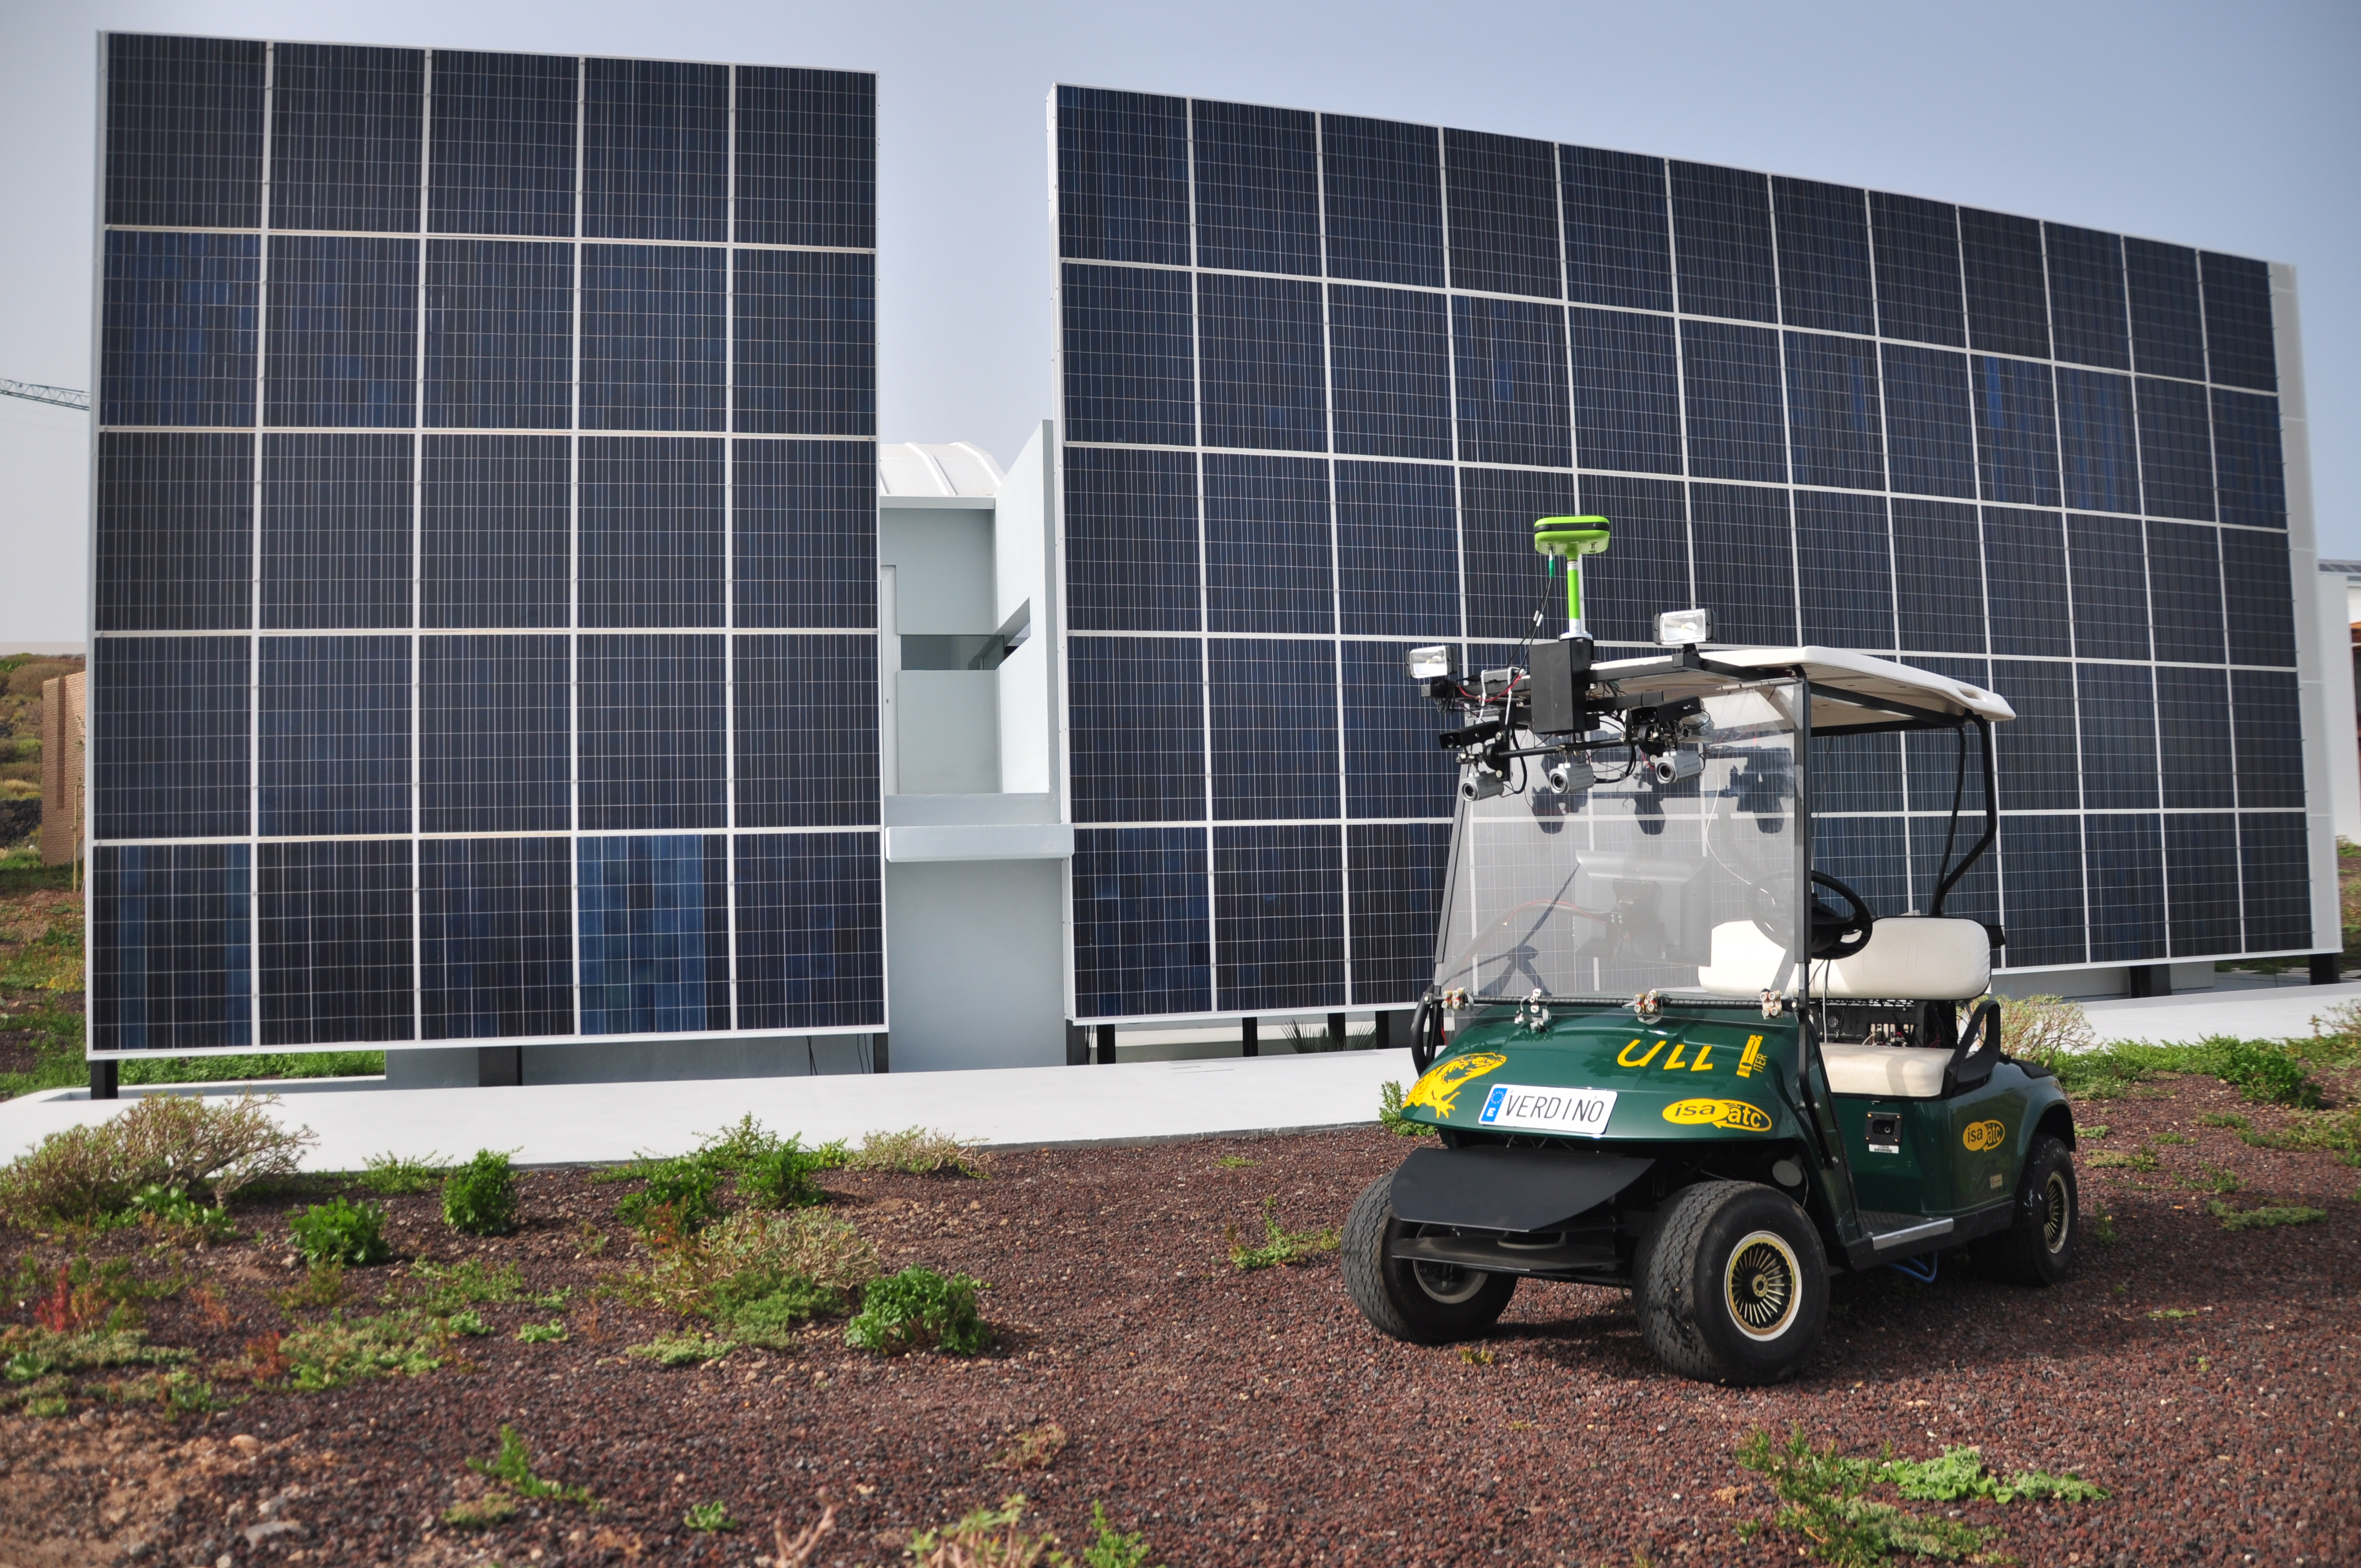
\includegraphics[height=\paperheight]{background}};\end{tikzpicture}}

% \setbeamercolor{alerted text}{fg=orange}
% \setbeamercolor{background canvas}{bg=green}
% \setbeamercolor{block body alerted}{bg=normal text.bg!90!black}
% \setbeamercolor{block body}{bg=normal text.bg!90!black}
% \setbeamercolor{block body example}{bg=normal text.bg!90!black}
% \setbeamercolor{block title alerted}{use={normal text,alerted text},fg=alerted text.fg!75!normal text.fg,bg=normal text.bg!75!black}
% \setbeamercolor{block title}{bg=blue}
% \setbeamercolor{block title example}{use={normal text,example text},fg=example text.fg!75!normal text.fg,bg=normal text.bg!75!black}
% \setbeamercolor{fine separation line}{}
% \setbeamercolor{frametitle}{fg=brown}
% \setbeamercolor{item projected}{fg=black}
% \setbeamercolor{normal text}{bg=black,fg=yellow}
% \setbeamercolor{palette sidebar primary}{use=normal text,fg=normal text.fg}
% \setbeamercolor{palette sidebar quaternary}{use=structure,fg=structure.fg}
% \setbeamercolor{palette sidebar secondary}{use=structure,fg=structure.fg}
% \setbeamercolor{palette sidebar tertiary}{use=normal text,fg=normal text.fg}
% \setbeamercolor{section in sidebar}{fg=brown}
% \setbeamercolor{section in sidebar shaded}{fg=gray}
% \setbeamercolor{separation line}{}
% \setbeamercolor{sidebar}{bg=red}
% \setbeamercolor{sidebar}{parent=palette primary}
% \setbeamercolor{structure}{bg=black, fg=green}
% \setbeamercolor{subsection in sidebar}{fg=brown}
% \setbeamercolor{subsection in sidebar shaded}{fg=gray}
% \setbeamercolor{title}{fg=brown}
% \setbeamercolor{titlelike}{fg=brown}

%% Video stuff
\usepackage{movie15}

% \AtBeginSubsection[]
% {
%   \begin{frame}
%     \frametitle{Table of Contents}
%     \tiny
%     \tableofcontents[currentsection]
%   \end{frame}
% }

\begin{document}
\addtobeamertemplate{headline}{}{%
\begin{textblock*}{100mm}(0.02cm,-0.8cm)

\includegraphics[height=.7cm]{verdino}
\end{textblock*}}

  \begin{frame}[plain]
    \centering
    
%     \includegraphics[height=0.5cm]{ull} \hspace*{0.5\textwidth}
%     
\includegraphics[height=2cm]{verdino} 
%     \begin{textblock*}{100mm}(0.02cm,-0.8cm)
%       
\includegraphics[height=.7cm]{verdino}
%     \end{textblock*}

    \titlepage
    
    \tiny
    \hfill Under the guidance of:\\
    \scriptsize
    \hfill Leopoldo Acosta Sánchez\\
    \hfill Jonay T. Toledo Carrillo

  \end{frame}

% \graphicspath{{./images/bmps/}{./images/vects/}{./images/}
  {./images/presentation/bmps/}{./images/presentation/vects/}{./images/presentation/}
  {./images/chapter00/bmps/}{./images/chapter00/vects/}{./images/chapter00/}
  {./images/chapter01/bmps/}{./images/chapter01/vects/}{./images/chapter01/}
  {./images/chapter02/bmps/}{./images/chapter02/vects/}{./images/chapter02/}
  {./images/chapter03/bmps/}{./images/chapter03/vects/}{./images/chapter03/}
  {./images/chapter04/bmps/}{./images/chapter04/vects/}{./images/chapter04/}
  {./images/chapter05/bmps/}{./images/chapter05/vects/}{./images/chapter05/}
  {./images/chapter06/bmps/}{./images/chapter06/vects/}{./images/chapter06/}
  {./images/chapter07/bmps/}{./images/chapter07/vects/}{./images/chapter07/}
}

\section{Introduction}
%   \begin{frame}{Introduction}
%     \begin{itemize}
%       \item<1-> Humans should not drive.
%       \begin{itemize}
% 	\item<2-> Road injuries are one of the top-ten causes death, according to the World Health Organization (WHO).
% 	\note {Fortunately, the number of deaths for this cause has been reduced.}
% 	\note {Popularization of Advanced Driver Assistance Systems (ADAS) could be very related to this fact.}
% 	\item<3-> Driving is difficult, too.
% 	\note{An average US citizen expends 38 hours stuck in traffic.}
%       \end{itemize}
%       \item<4-> The amount of research related to autonomous vehicles has increased a lot.
%     \end{itemize}  
%     \begin{center}
%       \includegraphics<1-1>[height=.45\textheight]{CarCartoon}
%       \includegraphics<2-2>[height=.45\textheight]{WHO-data-10-deaths}
%       \includegraphics<3-3>[height=.45\textheight]{trafficsigns}
%       \includegraphics<4-4>[height=.45\textheight]{uav_research}
%     \end{center}
%   \end{frame}
  
%   \begin{frame}{Advantages of autonomous vehicles}
%     \begin{columns}[c] % the "c" option specifies center vertical alignment
%       \column{.5\textwidth} % column designated by a command
%       \begin{itemize}
% 	\item<1-> Higher safety.      
% 	\item<2-> Reduced traffic congestion.
% 	\item<3-> More free time.
% 	\item<4-> Higher speed limits.
% 	\item<5-> Occupant constraints.
% 	\item<6-> Parking problems.
% 	\item<7-> Traffic police.
% 	\item<8-> Vehicle insurance.
% 	\item<9-> Road signs.
% 	\item<10-> Smoother ride.
%       \end{itemize}  
%       \column{.5\textwidth}
%       \begin{center}
% 	\includegraphics<1-1>[width=\textwidth]{safety}
% 	\includegraphics<2-2>[width=\textwidth]{congestion}
% 	\includegraphics<3-3>[width=\textwidth]{freetime}
% 	\includegraphics<4-4>[width=\textwidth]{speedlimit}
% 	\includegraphics<5-5>[width=\textwidth]{stpatricks}
% 	\includegraphics<6-6>[width=\textwidth]{parking}
% 	\includegraphics<7-7>[width=\textwidth]{police}
% 	\includegraphics<8-8>[width=\textwidth]{insurance}
% 	\includegraphics<9-9>[width=\textwidth]{roadsign}
% 	\includegraphics<10-10>[width=0.8\textwidth]{smoothride}
%       \end{center}
%     \end{columns}
%     
%     \note {
%     \begin{itemize}
%       \item As said, higher safety due a to a decrease in the number of traffic accidents.
%       \item Reduced traffic congestion, as the roads can increase their capacity.
%       \item Vehicle occupants can spend their time in things other than driving.
%       \item Higher speed limits.
%       \item Occupants are not tied to constraints like being under age, blind, intoxicated, etc.
%       \item Alleviation of parking scarcity and reduction of space required for vehicle parking.
%       \item Reduction in the need for traffic police and vehicle insurance.
%       \item Physical road signs will not be needed anymore: autonomous cars could receive necessary communication electronically.
%       \item Smoother ride.
%     \end{itemize}
%     }
%   \end{frame}

  \subsection{Problem Statement}
  \begin{frame}{Problem Statement}
    \begin{itemize}
     \item<1-> We propose different methods which will be used for the detection and tracking of obstacles by our prototype, Verdino.
     \item<2-> These will be used by a global and a local planner for generating and following a safe path.
    \end{itemize}
    \begin{center}
      \includegraphics<1->[height=.35\columnwidth]{verdino}
    \end{center}
  \end{frame}
  
  \begin{frame}[plain]{Pipeline}
    \begin{center}
      \includegraphics[height=1.1\textheight]{pipeline_cp0}
    \end{center}
    
  \end{frame}

  
  \begin{frame}{Obstacle detection and tracking}
    \begin{itemize}
    \item<1-> Goals:
      \begin{enumerate}
      \item<2-> Good obstacle detection rate. 
      \item<3-> Obstacle localization.
      \item<4-> Real time.
      \item<5-> Environment conditions independence.
      \item<6-> Tracking capabilities.
      \item<7-> Moving cameras.
      \end{enumerate}
    \end{itemize}
  \end{frame}
  
%   \begin{frame}{Obstacle detection and tracking}
%     \begin{itemize}
%       \item <1-> We propose four different approaches:
%       \begin{enumerate}
% 	\item<1-> Change detection and image registration. 
% 	\item<2-> Background substraction and nonrigid point set registration.
% 	\item<3-> Stixels.
% 	\item<4-> Voxels and a particle filter.
%       \end{enumerate}
%     \end{itemize}
%       
%     \begin{center}
%       \includegraphics<1-1>[height=.3\columnwidth]{database}
%       \includegraphics<2-2>[height=.3\columnwidth]{fig6}
%       \includegraphics<3-3>[height=.3\columnwidth]{stixels_over_original}
%       \includegraphics<4-4>[height=.3\columnwidth]{fakePointCloud}
%     \end{center}
%   \end{frame}
  
  \begin{frame}{Obstacle Avoidance and Planning}
    We distinguish two different levels:
    \begin{enumerate}
     \item<1-> Global planning. 
     \item<2-> Local planning.
    \end{enumerate}

    \begin{center}
      \includegraphics<1-1>[height=.35\columnwidth]{figure7}
      \includegraphics<2-2>[height=.35\columnwidth]{example3a}
    \end{center}
  \end{frame}
  
  \begin{frame}{Evaluation of Stereo 3D Reconstruction Algorithms}
    Apart from the previous, we developed some methods intended to assess the performance of the 3D stereo reconstruction algorithms used for the particle filter based approach.
    
    \begin{center}
      \includegraphics[height=.4\columnwidth]{fc}
    \end{center}
    
  \end{frame}
    
  \subsection{Previous Work}
%   \begin{frame}{Autonomous vehicles review}
%     \begin{columns}[T] % the "c" option specifies center vertical alignment
%       \column{.5\textwidth} % column designated by a command
%       \footnotesize
%       \begin{itemize}
% 	\item<1-> \textbf{(1987-1995)} EC EUREKA Prometheus Project.
% 	\item<2-> \textbf{(1996)} ARGO Project.
% 	\item<3-> \textbf{(2004)} $1^{st}$ DARPA's Grand Challenge.
% 	\item<4-> \textbf{(2005)} $2^{nd}$ DARPA's Grand Challenge.
% 	\item<5-> \textbf{(2007)} DARPA's Urban Challenge.
% 	\item<6-> \textbf{(2010, 2012, 2013)} Korean Autonomous Vehicle Competition (AVC).
%       \end{itemize}  
%       \column{.5\textwidth}
%       \begin{center}
% 	\vskip -1cm
%        	\begin{overlayarea}{\textwidth}{\textheight}
% 	  \only<1>{
% 	  \begin{block}{EC EUREKA Project}
% 	    \begin{itemize}
% 	    \item VITA-2\\
% 	    \begin{center}\includegraphics<1->[width=0.5\textwidth]{vita2}\end{center}
% 	    \item VaMP\\
% 	    \begin{center}\includegraphics<1->[width=0.5\textwidth]{VaMP}\end{center}
% 	    \end{itemize}
% 	  \end{block}
% 	  }
% 	  \only<2>{
% 	  \begin{block}{ARGO Project}
% 	    \begin{itemize}
% 	      \item Lancia Thema.
% 	      \item Follow the lane marks of a road.
% 	      \item 1,900\,km
% 	      \item Average of 60\,Km/h.
% 	    \end{itemize}
% 	    \begin{center}\includegraphics<1->[width=0.5\textwidth]{argo}\end{center}
% 	  \end{block}
% 	  }
% 	  \only<3>{
% 	  \begin{block}{$1^{st}$ DARPA's Grand Challenge}
% 	    \begin{itemize}
% 	      \item Mojave Desert.
% 	      \item 240\,km route.
% 	      \item Listing of check points.
% 	      \item None finished the route.
% 	    \end{itemize}
% 	    \begin{center}\includegraphics<1->[width=0.5\textwidth]{urbanchallenge2004}\end{center}
% 	  \end{block}
% 	  }
% 	  \only<4>{
% 	  \begin{block}{$2^{nd}$ DARPA's Grand Challenge}
% 	    \begin{figure}[t]
% 		    \centering
% 		    \begin{subfigure}[b]{0.4\textwidth}
% 		      \includegraphics[width=\textwidth]{stanley}
% 		    \end{subfigure}
% 		    ~
% 		    \begin{subfigure}[b]{0.4\textwidth}
% 		      \includegraphics[width=\textwidth]{Sandstorm}
% 		    \end{subfigure}
% 		    \\~\\
% 		    \begin{subfigure}[b]{0.4\textwidth}
% 		      \includegraphics[width=\textwidth]{h1ghlander}
% 		    \end{subfigure}
% 		    ~
% 		    \begin{subfigure}[b]{0.4\textwidth}
% 		      \includegraphics[width=\textwidth]{kat5}
% 		    \end{subfigure}
% 		    \\~\\
% 		    \begin{subfigure}[b]{0.4\textwidth}
% 		      \includegraphics[width=\textwidth]{terramax}
% 		    \end{subfigure}
% 	    \end{figure}
% 	  \end{block}
% 	  }
% 	  \only<5>{
% 	  \begin{block}{DARPA's Urban Challenge}
% 	    \begin{figure}[t]
% 		    \centering
% 		    \begin{subfigure}[b]{0.4\textwidth}
% 		      \includegraphics[width=\textwidth]{boss}
% 		    \end{subfigure}
% 		    ~
% 		    \begin{subfigure}[b]{0.4\textwidth}
% 		      \includegraphics[width=\textwidth]{junior}
% 		    \end{subfigure}
% 		    \\~\\
% 		    \begin{subfigure}[b]{0.4\textwidth}
% 		      \includegraphics[width=\textwidth]{odin}
% 		    \end{subfigure}
% 		    ~
% 		    \begin{subfigure}[b]{0.4\textwidth}
% 		      \includegraphics[width=\textwidth]{talos}
% 		    \end{subfigure}
% 		    \\~\\
% 		    \begin{subfigure}[b]{0.4\textwidth}
% 		      \includegraphics[width=\textwidth]{littleben}
% 		    \end{subfigure}
% 		    ~
% 		    \begin{subfigure}[b]{0.4\textwidth}
% 		      \includegraphics[width=\textwidth]{skynet}
% 		    \end{subfigure}
% 
% 	    \end{figure}
% 	  \end{block}
% 	  }
% 	  \only<6>{
% 	  \begin{block}{Korean Autonomous Vehicle Competition (AVC)}
% 	    \includegraphics[width=\textwidth]{kavc}
% 	  \end{block}
% 	  }
% 	\end{overlayarea}
%       \end{center}
%     \end{columns}
%     
%     \note {
%     \begin{itemize}
%       \item From 1987 to 1995, the EC EUREKA Prometheus Project conducted research on autonomous vehicles. Among its culmination points were the twin robot vehicles VITA-2 and VaMP, driving long distances in heavy traffic.
%       \item In 1996, the ARGO project modified a Lancia Thema to follow the lane marks in an unmodified highway \citep{Broggi1999}. The culmination of the project was a journey of 1,900\,km over six days on the motorways of northern Italy, with an average speed of 90 km/h. The car operated in fully automatic mode for the 94\% of its journey, with the longest automatic stretch being 55\,km. The vehicle had only two grayscale low-cost video cameras on board and used stereoscopic vision algorithms to understand its environment. 
%       \item In 2004, DARPA's Grand Challenge was held in the Mojave Desert region of the United States, along a 240\,km route. This competition consisted on an autonomous vehicles race that must reach to the goal without human intervention and using just a listing of check points between the start and the finish line. None of the robot vehicles finished the route.
%       \item In 2005, a second competition was held \citep{Buehler2007}. This time, five vehicles successfully completed the course:
%       \begin{itemize}
%       \item \emph{Stanley} \citep{thrun2006stanley}, from Standford University.
%       \item \emph{Sandstorm} and \emph{H1ghlander} \citep{urmson2004high}, from the Carnegie Mellon University.
%       \item \emph{Kat-5} \citep{trepagnier2006kat}, from the Gray Insurance Company.
%       \item \emph{TerraMax} \citep{ozguner2004team}, from the Oshkosh Truck Corporation.
%       \end{itemize}
%       \item In 2007, the third driverless car competition of the DARPA Grand Challenge \citep{Buehler2009}, more known as the DARPA Urban Challenge, was held in Victorville, California. This time, six teams successfully finished the entire course:
%       \begin{itemize}
%       \item \emph{Boss} \citep{Urmson2008}, from the Carnegie Mellon University.
%       \item \emph{Junior} \citep{montemerlo2008junior}, from Standford University.
%       \item \emph{Odin} \citep{Bacha2008}, from Virginia Tech.
%       \item \emph{Talos} \citep{leonard2007team}, from the Massachusetts Institute of Technology.
%       \item \emph{Little Ben} \citep{bohren2008little}, from University of Pennsylvania.
%       \item \emph{Skynet} \citep{miller2008team}, from Cornell University.
%       \end{itemize}
%       \item In 2010, 2012 and 2013, the Korean Autonomous Vehicle Competition (AVC) took place.
%     \end{itemize}
%     }
%   \end{frame}
% 
%   \begin{frame}{Autonomous vehicles review}
%     \begin{columns}[T] % the "c" option specifies center vertical alignment
%       \column{.5\textwidth} % column designated by a command
%       \footnotesize
%       \begin{itemize}
% 	\item<1-> \textbf{(2010)} VIAC Challenge.
% 	\item<3-> \textbf{(2011)} WildCat Project.
% 	\item<4-> \textbf{(2011)} AutoNOMOS Group.
% 	\item<5-> \textbf{(2012)} Shelley.
% 	\item<6-> \textbf{(February 2013)} RobotCar project.
% 	\item<7-> \textbf{(July 2013)} BRAiVE.
% 	\item<8-> \textbf{(Nowadays)} Many working prototypes.
%       \end{itemize}  
%       \column{.5\textwidth}
%       \begin{center}
% 	\vskip -1cm
%        	\begin{overlayarea}{\textwidth}{\textheight}
% 	  \only<1-2>{
% 	  \begin{block}{VIAC Challenge}
% 	    \begin{itemize}
% 	    \item<1-> From Italy to China.
% 	    \item<1-> 100 day, 15,900\,km.
% 	    \item<2-> Four autonomous vehicles.
% 	    \item<2-> Limited human intervention.
% 	    \end{itemize}
% 	    \begin{center}
% 	      \includegraphics<1>[width=0.8\textwidth]{viacMap}
% 	      \includegraphics<2>[width=0.8\textwidth]{viacCars}
% 	    \end{center}
% 
% 	  \end{block}
% 	  }
% 	  \only<3>{
% 	  \begin{block}{WildCat Project}
% 	    \begin{itemize}
% 	      \item Bowler Wildcat.
% 	      \item Oxford University.
% 	    \end{itemize}
% 	    \begin{center}\includegraphics<1->[width=\textwidth]{wildcat}\end{center}
% 	  \end{block}
% 	  }
% 	  \only<4>{
% 	  \begin{block}{AutoNOMOS Group}
% 	    \begin{itemize}
% 	      \item Spirit of Berlin.\\
% 	      \begin{center}\includegraphics<1->[width=0.5\textwidth]{spiritofberlin}\end{center}
% 	      \item MadeInGermany.\\
% 	      \begin{center}\includegraphics<1->[width=0.5\textwidth]{madeingermany}\end{center}
% 	    \end{itemize}
% 	  \end{block}
% 	  }
% 	  \only<5>{
% 	  \begin{block}{Shelley}
% 	    \begin{itemize}
% 	      \item More than 160\,km/h
% 	    \end{itemize}
% 	    \begin{center}\includegraphics<1->[width=\textwidth]{shelley}\end{center}
% 	  \end{block}
% 	  }
% 	  \only<6>{
% 	  \begin{block}{RobotCar project}
% 	    \begin{itemize}
% 	      \item Oxford University.
% 	      \item Switches from manual to autopilot on learned routes.
% 	    \end{itemize}
% 	    \includegraphics[width=\textwidth]{robotcar}
% 	  \end{block}
% 	  }
% 	  \only<7>{
% 	  \begin{block}{BRAiVE}
% 	    \begin{itemize}
% 	      \item Vislab.
% 	      \item Moved on a mixed traffic route open to public traffic.
% 	    \end{itemize}
% 	    \includegraphics[width=\textwidth]{BRAiVE}
% 	  \end{block}
% 	  }
% 	  \only<8>{
% 	  \begin{block}{Many working prototypes}
% 	    \begin{figure}[t]
% 	      \centering
% 	      \begin{subfigure}[b]{0.2\textwidth}
% 		\includegraphics[width=\textwidth]{mercedes_benz}
% 	      \end{subfigure}
% 	      ~
% 	      \begin{subfigure}[b]{0.2\textwidth}
% 		\includegraphics[width=\textwidth]{gm}
% 	      \end{subfigure}
% 	      ~
% 	      \begin{subfigure}[b]{0.2\textwidth}
% 		\includegraphics[width=\textwidth]{continental}
% 	      \end{subfigure}
% 	      \\~\\
% 	      \begin{subfigure}[b]{0.2\textwidth}
% 		\includegraphics[width=\textwidth]{autoliv}
% 	      \end{subfigure}
% 	      ~
% 	      \begin{subfigure}[b]{0.2\textwidth}
% 		\includegraphics[width=\textwidth]{bosch}
% 	      \end{subfigure}
% 	      ~
% 	      \begin{subfigure}[b]{0.2\textwidth}
% 		\includegraphics[width=\textwidth]{nissan}
% 	      \end{subfigure}
% 	      \\~\\
% 	      \begin{subfigure}[b]{0.2\textwidth}
% 		\includegraphics[width=\textwidth]{toyota}
% 	      \end{subfigure}
% 	      ~
% 	      \begin{subfigure}[b]{0.2\textwidth}
% 		\includegraphics[width=\textwidth]{audi}
% 	      \end{subfigure}
% 	      ~
% 	      \begin{subfigure}[b]{0.2\textwidth}
% 		\includegraphics[width=\textwidth]{vislab_logo}
% 	      \end{subfigure}
% 	      \\~\\
% 	      \begin{subfigure}[b]{0.2\textwidth}
% 		\includegraphics[width=\textwidth]{oxforduni_logo}
% 	      \end{subfigure}
% 	      ~
% 	      \begin{subfigure}[b]{0.2\textwidth}
% 		\includegraphics[width=\textwidth]{google}
% 	      \end{subfigure}
% 	    \end{figure}
% 	  \end{block}
% 	  }
% 	\end{overlayarea}
%       \end{center}
%     \end{columns}
%     
%     \note {
%     \begin{itemize}
%       \item In 2010, inside the VIAC Challenge, four autonomous vehicles drove from Italy to China on a 100-day 15,900\,km trip with only limited human intervention (in traffic jams and when passing toll stations). At the time, this was the longest-ever journey conducted by an unmanned vehicle \citep{Broggi2010VIAC}.
%       \item In 2011, under the Oxford University's WildCat Project, a Bowler Wildcat based prototype is capable of autonomous operation using a flexible and diverse sensor suite.
%       \item In 2011, the Freie Universität Berlin, Led by the AutoNOMOS group, developed two autonomous cars - \emph{Spirit of Berlin} \citep{berlin2007spirit} and \emph{MadeInGermany} \citep{gohring2013semi} - to drive in the innercity traffic of Berlin in Germany. They were able to handle intercity traffic, traffic lights and roundabouts between the International Congress Centrum and the Brandenburg Gate.
%       \item In 2012, Stanford's Dynamic Design Lab, in collaboration with the Volkswagen Electronics Research Lab, produced Shelley, an Audi TTS designed for high speed (greater than 160\,km/h) on a racetrack course.
%       \item In February 2013, Oxford University unveiled the RobotCar UK project, an inexpensive autonomous car capable of quickly switching from manual driving to autopilot on learned routes.
%       \item In July 2013, Vislab worldpremiered BRAiVE, a vehicle that moved autonomously on a mixed traffic route open to public traffic \citep{grisleri2010braive}.
%       \item Currently, many major companies and research organizations have developed working prototype autonomous vehicles, including Mercedes-Benz, General Motors, Continental Automotive Systems, Autoliv Inc., Bosch, Nissan, Toyota, Audi, Vislab (University of Parma), Oxford University and Google.
%     \end{itemize}
%     }
%   \end{frame}
  
  \begin{frame}[plain]{Obstacle detection}
    \begin{overlayarea}{\textwidth}{\textheight}
      \only<1-7> {
	We can divide object tracking methods into two subcategories:
	\begin{itemize}
	  \item \emph{2.5D Solutions:} Different approaches:
	  \begin{itemize}
	    \item \emph{6D Vision.} \cite{franke20056d}
	    \item \emph{Dynamic stixels.} \cite{badino2009stixel, pfeiffer2011towards, pfeiffer2013exploiting, benenson2011stixels, benenson2012pedestrian, benenson2012fast}
	    \item \emph{Tracked image features.} \cite{barth2009estimating}
	    \item \emph{Sensor fusion.} \cite{wu2009collision}
	    \item \emph{Occupancy grids.} \cite{danescu2012particle}
	  \end{itemize} 
	  \item \emph{3D Solutions}
	  \begin{itemize}
	    \item \emph{Voxel grids.} \cite{broggi2013}
	    \item \emph{Adjacent stacks of cells} \cite{Moravec96robotspatial}
	  \end{itemize}
	\end{itemize}
      }
    \end{overlayarea}
    \begin{overlayarea}{\textwidth}{\textheight}
      \only<2> {
	\vspace{-4.5cm}
	\begin{block}{6D-Vision}
	  \begin{center}
	    \includegraphics[height=0.5\textheight]{6dvision}
	  \end{center}
	\end{block}
      }
      \only<3> {
	\vspace{-4.5cm}
	\begin{block}{Stixel World}
	  \begin{center}
	    \includegraphics[height=0.5\textheight]{stixels_over_original}
	  \end{center}
	\end{block}
      }
      \only<5> {
	\vspace{-3cm}
	\begin{block}{Occupancy grids}
	  \begin{center}
	    \includegraphics[width=\textwidth]{danescuPF}
	  \end{center}
	\end{block}
      }
      \only<6> {
	\vspace{-8.2cm}
	\begin{block}{Voxel Grids}
	  \begin{center}
	    \includegraphics[height=0.4\textheight]{vislabVoxel}
	  \end{center}
	\end{block}
      }
    \end{overlayarea}
    \note{
    Based on how much information they use, we can divide object tracking methods into two subcategories:
    \begin{itemize}
      \item \emph{2.5D Solutions:} They do not make use of the complete information provided by 3D points. Instead of that, they tend to use elevation maps composed of uniform size cells. Each cell just stores occupancy and height information. This is the kind of methods that, as described before, usually consider obstacles as being in contact with a flat ground.
      In these methods, tracking is performed before the complete reconstruction is done, in an intermediate point based on an specific feature. Depending on the feature used, we distinguishing different approaches:
      \begin{itemize}
	\item \emph{Use of the 3D point as feature.} An example of this is the so called 6D vision \citep{franke20056d}, in which the 3D stereo vision extracted information is combined with an efficient implementation of an optical flow in the image space based on a GPU. Relevant points are tracked using a Kalman filter.
	\item \emph{Dynamic stixels.} This approach has been longer discussed in section \ref{ch:chapter00_02_04}.
	\item \emph{Tracked image features.} An example is the work by \cite{barth2009estimating}. There, obstacles are represented as a rigid 3D point set which are tracked in terms of feature displacements and depth measurements.
	\item \emph{Sensor fusion.} \cite{wu2009collision} reconstruct the objects as cuboids from a stereo point cloud. In this process, position and speed values are improved to a very accurate value by the use of a radar along with stereo.
	\item \emph{Occupancy grids.} This is a very popular choice for tracking. An occupancy grid is a probabilistic map of the driving environment, which encodes the past and present knowledge from sensor data, and which can be updated dynamically when new information is available. These occupancy grids can be cartesian, with rectangular cells, polar, or even a relation between columns in an image and the disparity. An example of this is the method by \cite{danescu2012particle}, which has inspired part of the work described in chapter \ref{ch:chapter05}.
	Another advantage of the model based on an occupancy grid is that it makes easier a collaborative update of the grid, which allows the usage of data from several sensors and observers. Another simple example of occupancy grid is that described in chapter \ref{ch:chapter07}.
      \end{itemize} 
      \item \emph{3D Solutions:} Usually based on complex grid maps that use complete 3D information. Again, depending on how this grid is represented, we find 
      \begin{itemize}
	\item \emph{Octree connected cubes.} An example is the work by \cite{wurm2010octomap} or \cite{broggi2013}.
	\item \emph{Adjacent stacks of cells}, as described in \cite{Moravec96robotspatial} 
      \end{itemize}
    \end{itemize}
    }
  \end{frame}

%   \begin{frame}{Path planning}
%     \begin{itemize}
%       \item Classical methods \citep{hwang1992gross}
%       \item Heuristic methods \citep{masehian2007classic}
%       \item SVM based methods
%       \begin{itemize}
%        \item Global
% 	 \begin{itemize}
% 	  \item \cite{miura2006support}
% 	  \item \cite{yang2012safe}
% 	 \end{itemize}
%        \item Local
% 	\begin{itemize}
% 	  \item \cite{sarkar2008mobile}
% 	  \item \cite{tennety2009support}
% 	  \item \cite{qingyang2012local}
% 	\end{itemize}
%       \end{itemize}
%     \end{itemize}
%     
%     \note{
%       About classical methods, in general they can be considered as variations of some general approaches: Roadmap, Cell Decomposition, Potential Fields and Mathematical Programming. These methods are not mutually exclusive; in fact, a lot of approaches use combinations of them. A review of some classical methods can be checked out in \cite{hwang1992gross}.
%  
%       About heuristic methods, these are the answer given by researchers to the limitations of the classic methods. The most representative methods inside this classification are Probabilistic Roadmaps (PRM) \citep{kavraki1996probabilistic}, Rapidly Exploring Random Trees (RRT) \citep{lavalle2000rapidly}, Level set \citep{sethian1999level}, Linguistic Geometry (LG) \citep{stilman1993network}, Simulated Annealing (SA) \citep{zhu2006robot}, Artificial Neural Network (ANN) \citep{hossain2012real}, Genetic Algorithms (GA) \citep{zhang2007evolutionary}, Particle Swarm Optimization (PSO) \citep{chen2006smooth}, Ant Colony (ACO) \citep{mou2008modified} and its variants, like the RNA algorithm described in \cite{zhu2011new}, Stigmergy \citep{cazangi2006evolutionary}, Wavelet Theory \citep{doh2005systematic}, Fuzzy Logic (FL) \citep{kladis2011energy} and Tabu Search (TS) \citep{nguyen2012multi}. For more information, the review in \cite{masehian2007classic} can be checked.
%       
%       Global:
%       In the work presented by \cite{miura2006support}, navigation is planned in environments in which the obstacles are known. Obstacles are randomly labeled into two classes: positive or negative. Using these two classes, a SVM is trained and the decision boundary is used as a path. To increase the efficiency, a set of fake obstacles (guide samples) is generated at both sides of the current and goal position, as well as in parallel to the line that joins both points (nominal line), with the objective of helping the SVM to find a feasible path.
%       \cite{yang2012safe}. In their work, a preprocessing step is used in which the Voronoi Diagram is generated using the obstacles in the map. That diagram is used to select the best path between the starting point of the robot and the goal. The path obtained using Voronoi is not smooth, so the SVM is used to make this path smoother. The SVM is trained using a dataset in which the sites that generated the Voronoi edges are classified as positive or negative depending on their position (left / right) regarding to the previously obtained path. The decision boundary of this SVM will be the final path used.
%       
%       Local:
%       In \cite{sarkar2008mobile, tennety2009support}, authors divide the whole set of objects in the map into two classes and the SVM is used to determine the maximum margin hyperplane between the data sets belonging to the two classes. Data is assigned to one or another class depending on whether the points are on the left or on the right side of the robot. Once the initial labels are assigned, further classification is done using the k-nearest neighbor algorithm, with k=1.
%       \cite{qingyang2012local}, that uses a path subdivision method and a SVM. They use topological maps of local environments which are extracted with little expanded nodes. Next, candidate routes are optimized using the Support Vector Machine, where the candidate routes boundary points are defined as positive and negative samples. They also extend the original SVM \citep{cortes1995support} in order to satisfy extra constraints such as vehicle position and heading.
%     }
%   \end{frame}
%   
%     \begin{frame}{Local planning}
%     \begin{itemize}
%       \item \cite{werling2010optimal}
%       \item \cite{thrun2006stanley}
%       \item \cite{chu2012local}
%     \end{itemize}
%      
%     \note{
%       \begin{itemize}
% 	\item In \cite{werling2010optimal}, long term objectives are performed, like speed keeping, merging, following, stopping. This is done through optimal control strategies within the Fren\'et frame of the street.
% 	\item In \cite{thrun2006stanley}, lateral offset is defined as the perpendicular to an established base trajectory. This allows the vehicle driving along the road parallel to this trajectory. In order to select the optimal path, the cost function penalizes passing over obstacles and the distance respect to the center of the current road.
% 	\item In \cite{chu2012local}, also a set of candidate paths are generated, with endpoints in fixed positions at different offsets respect to the base frame, but they do not set this base frame in the center of the road, since it could be dangerous when computing the costs at certain scenarios. Instead of that, they use a security cost for each candidate path. Security of the path is computed by blurring the binary data of the obstacles. They also have into account certain criteria, as the smoothness cost or the path consistency between iterations.
%       \end{itemize}
%     }
%   \end{frame}
  
  \subsection{Testing platform}
  \begin{frame}{Testing platform}
    These algorithms are intended to be used in Verdino.
    \begin{itemize}
     \item<1-> Prototype developed by GRULL, Universidad de La Laguna.
     \item<2-> It will transport people around a bioclimatic urbanization in the ITER facilities.
     \item<3-> A golf cart has been modified to be used as an unmanned vehicle.
    \end{itemize}

    \begin{center}
      \includegraphics<1-1>[height=.3\columnwidth]{verdino}
      \includegraphics<2-2>[height=.3\columnwidth]{iter}
      \includegraphics<3-4>[height=.3\columnwidth]{NV_TXT2}
      \includegraphics<4-4>[height=.3\columnwidth]{verdino}
    \end{center}
  \end{frame}
  
%   \begin{frame}{Actuators}
%     \begin{columns}[c] % the "c" option specifies center vertical alignment
%       \column{.5\textwidth} % column designated by a command
%       \begin{itemize}
% 	\item<1-> Steering system.      
% 	\item<2-> Braking system.
% 	\item<3-> Speed system.
% 	\item<4-> Safety switch.
%       \end{itemize}  
%       \column{.5\textwidth}
%       \begin{center}
% 	\includegraphics<1-1>[width=\textwidth]{steering}
% 	\includegraphics<2-2>[width=\textwidth]{braking}
% 	\includegraphics<3-3>[width=\textwidth]{speedControl}
% 	\includegraphics<4-4>[width=\textwidth]{panicbutton}
%       \end{center}
%     \end{columns}
%     
%     \note {
%     \begin{itemize}
%       \item Steering system: we tied the original steering to a DC motor controlled by a PID.
%       \item Braking system: Controlled through a pneumatic system, composed by a cylinder, a commutation valve, two flow controllers and an air compressor. The pneumatic cylinder acts over the brake cables, that make pressure over the brake drums. A compressor gives the air pressure needed for this process.
%       \item Speed system: A microcontroller generates three different signals, that simulate the original devices installed in the vehicle. These correspond to a switch relay, which turns on the motor when the user pushes the acceleration pedal; the sense of speed (forward or backward); and the desired voltage
%       \item Safety switch: Allows changing between automatic and manual behavior. When switched off, the vehicle behaves as it was before the modifications.
%     \end{itemize}
%     }
%   \end{frame}
% 
%   \begin{frame}{Sensors}
%     \begin{columns}[c] % the "c" option specifies center vertical alignment
%       \column{.5\textwidth} % column designated by a command
%       \begin{itemize}
% 	\item<1-> Localization sensors.      
% 	\begin{itemize}
% 	  \item<3-> Odometry.      
% 	  \item<4-> IMU.
% 	  \item<5-> Differential GPS.
% 	\end{itemize}  
% 	\item<2-> Navigation sensors.	
% 	\begin{itemize}
% 	  \item<6-> LIDAR.      
% 	  \item<7-> IR cameras.
% 	  \item<8-> Visible cameras.
% 	\end{itemize}
%       \end{itemize}  
%       \column{.5\textwidth}
%       \begin{center}
% 	\includegraphics<3-3>[width=\textwidth]{odometry}
% 	\includegraphics<4-4>[width=\textwidth]{imu}
% 	\includegraphics<5-5>[width=\textwidth]{dgps}
% 	\includegraphics<6-6>[width=\textwidth]{lidar}
% 	\includegraphics<7-7>[width=\textwidth]{ircameras}
% 	\includegraphics<8-8>[width=\textwidth]{visiblecamera}
%       \end{center}
%     \end{columns}
%     
%     \note {
%     \begin{itemize}
%       \item \emph{Odometry}: This system measures the independent movement of the two rear wheels, which are attached to an optical encoder. This allows computing the position, orientation and speed of the prototype incrementally.
%       \item \emph{IMU}: It is comprised by 9 sensors (3 accelerometers, 3 gyroscopes and 3 magnetometers), which are fused in real time in order to get the three-dimensional orientation of the vehicle. The model of the sensor is a \emph{Xsens Mti}.
%       \item \emph{DGPS}: Allows positioning the vehicle with centimetric accuracy. It is composed by two different devices, the reference station, which is fixed in a known place, and the rover station, which is installed on the vehicle. The model used is a \emph{JAVAD GNSS Triumph-1}, which has an horizontal precision below 1\,cm and a vertical precision around 1.5\,cm using DGPS, at a frequency of $5\,Hz$.
%       \item \emph{LIDAR}: These are used also for localization purposes. Each of those sensors is able to detect the objects in the way of the vehicle, at the plane in which the sensor is mounted. The advantages of these sensors are that they have a high speed and precision. However, they are just able to detect obstacles that crosses the plane defined by the sensor. Because of this, we have equipped the vehicle with 5 LIDAR. Two of them are located at the same plane in the front corners of the vehicle, at a height of 50\,cm. Each of these covers an angle of 270\textdegree. Another is located in the front side of the vehicle, at a height of 20\,cm, slightly tilted upwards, in order to detect the small obstacles or non traversable areas. Another is in the top of the vehicle, also in the front side of the vehicle, tilted to the ground and covering the blind areas left by the other sensors. Finally, the last sensor is situated in the back side of the vehicle, and it is used for backwards maneuvers. The used sensors are of the model \emph{SICK LMS 100} and \emph{SICK LMS 111}, allowing a maximal detection distance of 20\,m, a precision of 10-35\,mm, a maximal angular resolution of 0.25\textdegree and a maximal rate of $50\,Hz$.
%       \item \emph{IR cameras}: Infrared cameras are used to detect pedestrians or animals based on their temperature. We have a pair of them installed on a Pan-Tilt system attached to the top front side of the vehicle. The model used is a \emph{MobiR\textregistered~M3}, which is able to detect objects in the range $8\sim14\mu m$, at a resolution of $160 \times 120\,px$.
%       \item \emph{Visible cameras}: A set of three cameras is also installed in a pan-tilt structure. These are used for the detection and tracking of the objects, which is one of the goals of this thesis. Also, they are currently being used for the detection of the borders of the road. The model of the cameras is a \emph{GoPro\textregistered Hero 3 silver edition}, with a $1920 \times 1080 \, px$ maximal video resolution and a 170\textdegree field of view at a maximal rate of 60\,fps.
%     \end{itemize}
%     }
%   \end{frame}
%   
%   \begin{frame}{Control}
%     \begin{columns}[c] % the "c" option specifies center vertical alignment
%       \column{.5\textwidth} % column designated by a command
%       \begin{itemize}
% 	\item Onboard computer.   
% 	\begin{itemize}
% 	  \item i7-3770K.      
% 	  \item 16 Gb RAM DDR3.
% 	  \item SSD Storage.
% 	\end{itemize}	
% 	\item Low-level control.
%       \end{itemize}  
%       \column{.5\textwidth}
%       \begin{center}
% 	\includegraphics[width=\textwidth]{onboard}
%       \end{center}
%     \end{columns}
%     
%     \note {
%     The vehicle is controlled, at high level, by an on board computer equipped with an \emph{i7-3770K} processor, 16\,Gb of \emph{RAM DDR-3} memory and a \emph{SSD} storage. At low level, a set of own developed electronic devices receive commands from the computer and transform them into the right signal, understandable by the actuators described before.
%     }
%   \end{frame}
  
\section{Obstacle Detection}
% %%
%%  chapter01.tex - Obstacle Detection and Planning for Autonomous Vehicles based on Computer Vision Techniques
%%
%%  Copyright 2014 Néstor Morales <nestor@isaatc.ull.es>
%%
%%  This work is licensed under a Creative Commons Attribution 4.0 International License.
%%

\chapter{Problem Statement}\label{ch:chapter01}

\section{Problem Statement}\label{ch:chapter01_01}

Computer Vision environment understanding targeted at enabling autonomous operation of a robotic platform has been widely studied over the years, leading to the creation of some prototype vehicles \cite{Maurer1996,Pomerleau1996,Broggi1999} which demonstrated that negotiating moderately complex and dynamic situations in real time was possible, albeit challenging. However, it was only with the development effort driven by the DARPA Challenges \cite{Buehler2007, Buehler2009} that the technology required to provide reliable operation both in off-road and urban scenarios proved to be within reach.
The vehicles that successfully took part to this series of events had to integrate planning and actuation capabilities with a sensing suite capable of coping with harsh environments, heavy traffic and wide temperature ranges, while keeping functional over extended amounts of time. Most competitors relied on high-end active sensors \cite{Urmson2008, Montemerlo2008, Bacha2008, Kammel2008}, with some notable exceptions \cite{Broggi2006, Broggi2010}. 

As we discover when looking up to the available literature (See next section, \ref{ch:chapter01_02}), there are many methods for the detection and tracking of obstacles in complex environments, like this for which Verdino is intended to be working. In this sense, a very first approach is that inspired on the work by \cite{primdahl2005change},  \cite{diego2011video} or \cite{vallespi2012prior} was developed. This is based on the fact that, in an image, a high percentage of the scene represented usually corresponds to static objects. Based on that, it looks quite straightforward to think that, having an image representing an area without obstacles, it is possible to detect the obstacles in an scene by just comparing it with an image being taken in real time. For that, we obtained a dataset with geo-referenced images from a closed urbanization taken at different times of the day. A description of this database, as well as of the algorithm pipeline used for the comparison between images pairs can be found at section \todo{ \ref{XXX} }.

However, such approach suffers from several drawbacks. First, as we just use one image per frame, we are no able to know the exact position of the obstacle in the real world \comment{(Anyway, we think that the output of the algorithm is a good starting point for a classification method)}. Also, the quality of detection is highly tied to the size of the image database, so in big areas we need a huge dataset, with the related space and throughput problems associated to that. If we consider changes due to weather or light conditions, this dataset grows exponentially. Finally, we don't know the direction where an obstacle is going to. These are challenging problems that have been solved using different approaches, until we reached a final solution, described in section \todo { \ref{XXX} }.

To solve that, we first developed a method that tries to isolate just the tracking problem with the use of static monocular cameras. Instead of registering pairs of images, we segment the image with the use of foreground extraction techniques, distinguishing between background and foreground. Using the silhouette of the objects in the foreground (which are mainly non-rigid objects, like pedestrians or animals), we apply a non-rigid point set registration algorithm in order to track the different parts of the body of the obstacles separately. This method, inspired in works like those by \cite{starck2007surface}, or \cite{letouzey2011scene}, can be also used for the completion of the global map of the vehicle, or even for tasks more related to \acf{HMI}. This approach is extensively described in section \todo{ \ref{XXX}}.

However, this method still makes use of a very rudimentary method for the localization of the obstacles (See section \todo{ \ref{XXX-subsection_localization}}), and it is limited to static cameras. For the application proposed, we need the cameras installed on the top of the moving prototype, so we can not use foreground segmentation methods anymore for the detection of the objects in the road. A simple solution for that is stop using monocular vision, and start using stereo vision. In the last years, a high number of advanced algorithms has become viable for autonomous driving applications. The problem is that performing a quantitative and meaningful comparison of their performance level, however, is not an easy task, mainly because of the difficulty of producing ground truth information. Older datasets are small, and either synthetic or taken in controlled environments (\cite{Scharstein2002}), thus effectively limiting their usefulness as indicators of the actual algorithms ability to cope with outdoor scenarios. Due to that, it is needed to compare the performance level of some state-of-the-art stereovision-based 3D mapping algorithms in automotive scenarios. This evaluation methodology and the associated results is shown in section \todo{ \ref{XXX}}. \comment{PREGUNTAR A LA GENTE DEL VISLAB SI ESTA DE ACUERDO CON QUE USE ESTO EN LA TESIS, POR SI LAS MOSCAS}.

\comment{Este párrafo y la sección asociada dependerá de lo que consiga sacar más adelante.}\notsure{
Apart from the full-dense 3D reconstruction methods, we also explore the possibility of using a simpler (and faster) reconstruction based on Stixels, like that described by \cite{badino2009stixel}. In particular, we decided to use the implementation by \cite{benenson2012pedestrian}, due to its fast response (about 100 frames per second). The method, described in section \todo{\ref{XXX}}, compares the stixels obtained between frames and tracks the obstacles along the time. This solves all the problems we had: we can use moving cameras, we can locate the obstacles in the map, and also we are able to know the path followed by them.}

Another approach, which makes use of the dense stereo reconstruction algorithms for which we did the evaluation described above, is inspired in the work by \cite{danescu2010particle}, but also from the voxelized world described in \cite{broggi2013}. The key idea is to simplify the 3d reconstructed world into a grid of voxels, each of these representing a certain volume in the world. In this voxelized world, for each voxel above a given occupancy probability threshold, a set of particles part of a particle filter is assigned. Each particle will have a double function: the first, denoting hypotheses (as in the classical particle filter methods); the second, to be used as segmentation criteria in the segmentation of the world into different obstacles. In this way, we consider that two contiguous voxels belong to different obstacles if their obtained direction and sense diverges. A more detailed explanation of the method is found in \todo{\ref{XXX}}.

At this point, we have an acceptable reconstruction of the surroundings of the vehicle, which includes the localization and tracking of the obstacles in the neighborhood of the cart. But the reconstruction of the environment is not the only challenge that an autonomous vehicle has to deal with. Once that a vehicle has an idea of where it is, and where it wants to go, it also needs to know the best way to reach there and, more important, how to avoid the harmful elements it has previously detected using the methods described. This allows a safe trip, both for the pedestrians, cars, etc. in the road, and for the vehicle itself.
As said, Verdino is intended to travel in pedestrian areas where most of the obstacles are pedestrians, so its behavior must be mainly reactive in order to give priority to the safety of paths against the efficiency of the route. Also, there is not a clear traveling path, like a road. Instead of that, the vehicle will be moving around an unstructured area, so there is not something like a \acf{RNDF} that allows a fast calculation of the paths that the car will use to reach a certain point. Because of that, we must consider two different planning levels:
\begin{itemize}
 \item \textbf{Global Planning:}
 As it is not possible to determine a global trajectory based on a \acs{RNDF}, we must use a method able to deal with changing environments for the calculation of a fast and safe path. The idea is that, having a map of the static obstacles in the environment and with the vehicle properly localized on it \cite{Perea2013mcl}, it will generate a path that will allow reaching this destination as fast as possible. This task, which can be solved easily in static environments using graphs or other similar optimization methods, becomes a little bit more challenging in environments like, for example, a parking lot, in which cars are parking and driving off continuously.
 In section \todo{ \ref{XXX} }, the way in which we solved this problem is described. It is based on the border between classes, which is obtained after training a \acf{MSVM} (See Appendix \todo {\ref{XXX}} for more information), considering each single obstacle as a separate class. Instead of using this border for classification purposes, as it is usual, we take advantage of the fact that it will be the safest and smoother distance to the obstacles. Taking this into account, it makes sense to apply this separation line as our path. Also, the use of a different class for each obstacle allows ensuring that the path is safe enough, even in complicate scenarios, like in pedestrian areas.
 
 \item \textbf{Local Planning:}
 In a lower level, we also need a way to make the vehicle know how to follow the generated path. This problem requires a system able to, several times per second, calculate the best steering angle and speed in order to follow the global plan while avoiding the surrounding obstacles. The method, which is inspired in the work of \cite{chu2012local}, receives as input the current position of the vehicle in the map, its orientation, speed and the steering angle. Also, we provide it with the global plan obtained in the upper level. Finally, a map of the dynamic obstacles in the surrounds of the cart is computed and passed to the algorithm.
 
 This dynamic map can be filled with the information provided by sensors like \acp{LIDAR}, among other sensors. But it can can also be computed with the information extracted from cameras, and this is the connection point with the work described in the first part of this Thesis. The detected obstacles are included in the map, so the vehicle is able to avoid them using the calculated steering angle and speed.
 
 The way in which both this map and the speed/steering angle commands is obtained is described in section \ref{XXX}.
\end{itemize}
 
 The whole pipeline of the application developed for this thesis is shown at figure \ref{fig:cp01_pipeline}. 
 
 \begin{figure}[thb]\label{fig:cp01_pipeline}
      \centering
      \includegraphics{pipeline}
      \caption{Pipeline of the modules described in this Thesis.}
\end{figure}

From the images captured in real-time, obstacles are located and passed to the module in charge of the generation of the dynamic costmap. At the same time, the static map is used for the generation of a feasible trajectory. Using the current position and vehicle status, the local planner tries to compute the proper commands in order to follow the global plan while trying to avoid the obstacles included in the dynamic costmap.

\section{Previous Work}\label{ch:chapter01_02}

Research on autonomous vehicles is a task being developed for a long time and for which a big effort has been carried on. A proof of that is the extensive literature existing about that topic, in special since the first of the DARPA Challenges (\cite{Buehler2007, Buehler2009}). Since then, the literature related to the topic has increased. Also, the interest on the use of Computer Vision in autonomous vehicles is growing, due to the possibilities that images offer when compared to other sensors, like \acp{LIDAR}.
In 1996, the ARGO project... \todo{Continuar desde aquí, una vez tenga una especie de historia de los vehiculos autonomos, en la intro.}
\todo{TerraMax, VIAC, Braive, Annieway y cualquier otro que pille por el camino.}
As depicted from section \ref{ch:chapter01_01}, the topics described in this thesis are quite diverse, so it is fair to review the state-of-the art of each of these topics separately.

\subsection{Change detection for obstacle localization in images}\label{ch:chapter01_02_01}

blah blah blah blah blah blah blah blah blah blah blah blah blah blah blah blah blah blah blah blah blah blah blah blah blah blah blah blah blah blah blah blah blah blah blah blah blah blah blah blah blah blah blah blah blah blah blah blah blah blah blah blah blah blah blah blah blah blah blah blah blah blah blah blah blah blah blah blah blah blah blah blah blah blah blah blah blah blah blah blah blah blah blah blah blah blah blah blah blah blah blah blah blah blah blah blah blah blah blah blah blah blah blah blah blah blah blah blah blah blah blah blah blah blah blah blah blah blah blah blah blah blah blah blah blah blah blah blah blah blah blah blah blah blah blah blah blah blah blah blah blah blah blah blah blah blah blah blah blah blah blah blah blah blah blah blah blah blah blah blah blah blah blah blah blah blah blah blah 

\subsection{Non-rigid point set registration for obstacle tracking}\label{ch:chapter01_02_02}

blah blah blah blah blah blah blah blah blah blah blah blah blah blah blah blah blah blah blah blah blah blah blah blah blah blah blah blah blah blah blah blah blah blah blah blah blah blah blah blah blah blah blah blah blah blah blah blah blah blah blah blah blah blah blah blah blah blah blah blah blah blah blah blah blah blah blah blah blah blah blah blah blah blah blah blah blah blah blah blah blah blah blah blah blah blah blah blah blah blah blah blah blah blah blah blah blah blah blah blah blah blah blah blah blah blah blah blah blah blah blah blah blah blah blah blah blah blah blah blah blah blah blah blah blah blah blah blah blah blah blah blah blah blah blah blah blah blah blah blah blah blah blah blah blah blah blah blah blah blah blah blah blah blah blah blah blah blah blah blah blah blah blah blah blah blah blah blah 

\subsection{Evaluation of stereo 3D reconstruction algorithms}\label{ch:chapter01_02_03}

blah blah blah blah blah blah blah blah blah blah blah blah blah blah blah blah blah blah blah blah blah blah blah blah blah blah blah blah blah blah blah blah blah blah blah blah blah blah blah blah blah blah blah blah blah blah blah blah blah blah blah blah blah blah blah blah blah blah blah blah blah blah blah blah blah blah blah blah blah blah blah blah blah blah blah blah blah blah blah blah blah blah blah blah blah blah blah blah blah blah blah blah blah blah blah blah blah blah blah blah blah blah blah blah blah blah blah blah blah blah blah blah blah blah blah blah blah blah blah blah blah blah blah blah blah blah blah blah blah blah blah blah blah blah blah blah blah blah blah blah blah blah blah blah blah blah blah blah blah blah blah blah blah blah blah blah blah blah blah blah blah blah blah blah blah blah blah blah 

\subsection{Stixel World}\label{ch:chapter01_02_04}

blah blah blah blah blah blah blah blah blah blah blah blah blah blah blah blah blah blah blah blah blah blah blah blah blah blah blah blah blah blah blah blah blah blah blah blah blah blah blah blah blah blah blah blah blah blah blah blah blah blah blah blah blah blah blah blah blah blah blah blah blah blah blah blah blah blah blah blah blah blah blah blah blah blah blah blah blah blah blah blah blah blah blah blah blah blah blah blah blah blah blah blah blah blah blah blah blah blah blah blah blah blah blah blah blah blah blah blah blah blah blah blah blah blah blah blah blah blah blah blah blah blah blah blah blah blah blah blah blah blah blah blah blah blah blah blah blah blah blah blah blah blah blah blah blah blah blah blah blah blah blah blah blah blah blah blah blah blah blah blah blah blah blah blah blah blah blah blah 

\subsection{3D object tracking}\label{ch:chapter01_02_05}

By processing the data captured by sensors, it is desired to obtain the position, speed and size of an obstacle. However, usually sensors don't provide this information, so we need to process the information over time and do the tracking of detected obstacles. Many approaches that try to solve this problem, like \cite{danescu2012particle}, assume that obstacles have an standard geometry, and they are modeled as cuboids with associated position, size and speed vectors. This assumption is mostly correct in environments like highways, country roads, and certain urban scenarios, in which almost all the obstacles are cars, trucks or buses which can be simplified as cuboids. Also, these approaches tend to consider a flat ground.
However, this assumption cannot always done, as happens in pedestrian areas, intersections, off-road... In this case, we need to deal with specific shapes, sometimes with concave surfaces. The problem with this kind of obstacles is that methods that assume cuboid-shaped objects tend to wrap the obstacles with a convex shape, which causes an overestimation of their volume (\cite{broggi2013}). Another problem are those objects that are not laying on the ground, as happens with hanged traffic lights, tree crowns, lamps, etc. Usually, they are integrated into an occupancy grid as if they were touching the ground. About the ground plane assumption, in cases like that of an off-road scenario, it is important to estimate the real slope of the road in order to get good results.
Based on how much information they use, we can divide object tracking methods into two subcategories:
\begin{itemize}
 \item \emph{2.5D Solutions:} They do not make use of the complete information provided by 3D points. Instead of that, they tend to use elevation maps composed of uniform size cells. Each cell just stores occupancy and height information. This is the kind of methods that, as described before, usually consider obstacles as being in contact with a flat ground.
 In these methods, tracking is done before the complete reconstruction is done, in an intermediate point based on an specific feature. Based on this intermediate feature, we can distinguishing different kind of approaches:
  \begin{enumerate}
   \item \emph{Use of the 3D point as feature.} An example of this is the so called 6D vision (\cite{franke20056d}), in which the 3D stereo vision extracted information is combined with an efficient implementation of an optical flow in the image space based on a \acf{GPU}. Relevant points are tracked using a Kalman filter.
   \item \emph{Dynamic stixels.} \todo{This approach has been longer discussed in section \ref{ch:chapter01_02_04}.}\comment{Cambiar en caso de que al final no meta los stixels}
   \item \emph{Tracked image features.} As example, check the work by \cite{barth2009estimating}. In this work, obstacles are represented as a rigid 3D point set which are tracked in terms of feature displacements and depth measurements.
   \item \emph{Sensor fusion.} \cite{wu2009collision} reconstruct the objects as cuboids from a stereo point cloud. In this process, position and speed values are improved to a very accurate value by the use of a radar along with stereo.
   \item \emph{Occupancy grids.} This is a very popular choice for tracking. An occupancy grid is a probabilistic map of the driving environment, which encodes the past and present knowledge from sensor data, and which can be updated dynamically when new information is available. These occupancy grids can be cartesian, with rectangular cells, polar, or even a relation between columns in an image an the disparity. An example of this is the method by \cite{danescu2012particle}, which has inspired part of the work described in section \todo { \ref{XXX}}.
   Another advantage of the model based on an occupancy grid is that it makes easier a collaborative update of the grid, which allows the usage of data from several sensors and observers.
  \end{enumerate} 
 \item \emph{3D Solutions:} Usually based on complex grid maps that use complete 3D information. Again, depending on how this grid is represented, we find 
 \begin{enumerate}
   \item \emph{Octree connected cubes.} An example is the work by \cite{wurm2010octomap} or \cite{broggi2013}.
   \item \emph{Adjacent stacks of cells}, as described in \cite{Moravec96robotspatial} 
 \end{enumerate}
\end{itemize}

\subsection{Global planning}\label{ch:chapter01_02_06}

blah blah blah blah blah blah blah blah blah blah blah blah blah blah blah blah blah blah blah blah blah blah blah blah blah blah blah blah blah blah blah blah blah blah blah blah blah blah blah blah blah blah blah blah blah blah blah blah blah blah blah blah blah blah blah blah blah blah blah blah blah blah blah blah blah blah blah blah blah blah blah blah blah blah blah blah blah blah blah blah blah blah blah blah blah blah blah blah blah blah blah blah blah blah blah blah blah blah blah blah blah blah blah blah blah blah blah blah blah blah blah blah blah blah blah blah blah blah blah blah blah blah blah blah blah blah blah blah blah blah blah blah blah blah blah blah blah blah blah blah blah blah blah blah blah blah blah blah blah blah blah blah blah blah blah blah blah blah blah blah blah blah blah blah blah blah blah blah 

\subsection{Local planning}\label{ch:chapter01_02_03}

blah blah blah blah blah blah blah blah blah blah blah blah blah blah blah blah blah blah blah blah blah blah blah blah blah blah blah blah blah blah blah blah blah blah blah blah blah blah blah blah blah blah blah blah blah blah blah blah blah blah blah blah blah blah blah blah blah blah blah blah blah blah blah blah blah blah blah blah blah blah blah blah blah blah blah blah blah blah blah blah blah blah blah blah blah blah blah blah blah blah blah blah blah blah blah blah blah blah blah blah blah blah blah blah blah blah blah blah blah blah blah blah blah blah blah blah blah blah blah blah blah blah blah blah blah blah blah blah blah blah blah blah blah blah blah blah blah blah blah blah blah blah blah blah blah blah blah blah blah blah blah blah blah blah blah blah blah blah blah blah blah blah blah blah blah blah blah blah 

\section{Summary}\label{ch:chapter01_03}

In this chapter, we have described a general idea of the work presented in this Thesis. Also, the pipeline of the final developed application is introduced. All this information will be explained in more detail in the following sections, including implementation details together with some results and a discussion of the advantages/disadvantages of the different methods.


% %%
%%  chapter02.tex - Obstacle Detection and Planning for Autonomous Vehicles based on Computer Vision Techniques
%%
%%  Copyright 2014 Néstor Morales <nestor@isaatc.ull.es>
%%
%%  This work is licensed under a Creative Commons Attribution 4.0 International License.
%%

\graphicspath{{./images/chapter02/bmps/}{./images/chapter02/vects/}{./images/chapter02/}}

\chapter{Change detection for obstacle localization in images}\label{ch:chapter02}

We drive by mind. That is, once we learn the path to go from a point $A$ to another point $B$, we follow that path without almost thinking. Even more, if a person does this way repeatedly and every day, there will be a day in which he will be able to memorize each black spot, each traffic light and even each pothole. So it is not difficult for us to be surprised the day in which they change the signals or the sense of a road.
Following this line of thought, we have developed a system in which we make our prototype to \emph{learn} the environment of a certain road, making it able to detect the changes. However, in our case, the changes in which we are interested are the obstacles in the way of the vehicle, giving it the ability to avoid them or to stop if necessary. The idea behind this system is having a dataset with images that have localization information associated. These images will be compared with those captured in real time by the on board cameras. Both images will be registered and changes detected, letting us to know the presence of obstacles or other changes that appeared since the stored images were captured.

This is done through the pipeline shown at figure \ref{fig:cp02_pipeline}. First, the database is captured offline. Then, in real time, images are aligned trough a typical image registration pipeline(feature localization, matching of the features between the images, image transformation and resampling). With the images aligned,  obstacles are retrieved.

\begin{figure}[thb]
  \centering
  \includegraphics{pipeline}
  \caption{Pipeline of the method.}
  \label{fig:cp02_pipeline}
\end{figure}

\section{The Method}\label{ch:chapter02_01}

In this section, we will describe each of the stages in the pipeline of the application, starting from the database generation and finishing with the detected obstacles. 

As said, the process is based on the generation of an image database in which each image is associated with certain meta-information, of which a big part is related to its position in the map, so the first step in the application is the development of a database covering the driving area. In this stage, the vehicle will be traveling inside the covered area, driven by a human or in controlled circumstances. While the vehicle is driven, the system stores images, which will have associated geographic information: \emph{latitude}, \emph{longitude}, \emph{height} and their transformation into $x$, $y$, $z$ and orientation coordinates with respect to the coordinates frame of the local map of the prototype. Other information that could be outstanding in the future is also stored (i.e., the day and the hour in which the image was taken, \ac{GPS} rms value, etc.). Images are pre-processed to have as information as possible when used in the next phase, reducing the execution times. For example, we get the set of features from the images offline, not in the real time application. With a $5\,Hz$ update rate, an image is stored about each meter traveled, depending on the speed of the vehicle. In this phase, there would not be any obstacle in the road where the car is going to drive. If so, in the later phase in which the images are processed to get the obstacles, fake objects are going to be detected, due to those obstacles recorded in the database image. Once this process is finished, there will be a database with geographically located images. In figure \ref{fig:cp02_image_database}, a composition of the testing area with some of the stored images highlighted is shown.

\begin{figure}[thb]
  \centering
  \includegraphics{database}
  \caption{Area covered by the database with some example images superimposed.}
  \label{fig:cp02_image_database}
\end{figure}

In real time, the vehicle starts driving by itself. Along the path, it passes over different positions near the recorded route. These positions are being reported by the \ac{GPS} device and transformed to the local coordinates to work easily with them. Simultaneously, an image is obtained from the camera while the system looks for the nearest image in the database. The current frame $I_{RT}$ and the image retrieved from the database $I_{DB}$ are compared by using image change detection techniques, obtaining the obstacles in the scene.

In the moment of the development of this application, localization was entirely retrieved from the \ac{GPS} device. This gave a position each 200 ms, so it was desirable to be able to process each frame under this time, in an on board 2009 PC computer.

\subsection{Image selection from database}\label{ch:chapter02_01_01}

This step is important as we want to get an image as similar as possible to the current real time image. This will affect to the quality of the adjustment between the images. Most of the times we just need to find an image with the smaller Euclidean distance to the current point, checking that the angular difference is not too big. Although this solution has good results, many times it is better to have an image not so close to the current point, if it means that all the objects represented in an image are going to appear in the other one. This can be got if an image which is forward or backward regarding to the current image is selected, so one of the images will be contained into the other. Doing that, it will reduce not just the angular difference, but also the lateral distance (which is usually the source of the misalignments due to an excess of parallax).

In figure \ref{fig:cp02_nearest_image}, we can observe this procedure. Based on this, the nearest image in the database is that obtained by the expression:

\begin{equation}\label{eq:cp02_nearest_image}
I^*_{DB} = \underset{I_{DB}}{\arg\min} \|p_{RT} - p_c\| = {{y_{RT} \cdot v_{DB_x} + x_{RT} \cdot v_{DB_y}} \over 
  {v_{DB_y} \cdot cos(\theta_{RT}) - v_{DB_x} \cdot sin(\theta_{RT})}}
\end{equation}

There, $p_{RT} = (x_{RT}, y_{RT})$ is the position of the vehicle, $p_{DB_i} = (x_{DB_i}, y_{DB_i})$ is the position of each of the images in the database, and $p_c = (x_c, y_c)$ is the crossing point shown at figure \ref{fig:cp02_nearest_image}; $v_{DB_x} = x_{DB} + cos(\theta_{DB})$ and $v_{DB_y} = y_{DB} + sin(\theta_{DB})$; and 
$\theta_{RT}$ and $\theta_{DB_i}$ are the orientations of the vehicle and each of the images in the database. At the end of this selection process a pair of images will be obtained: the current frame, and the associated image extracted from the database. At the same time, we get other related information from the database, like masks, control points, and other things previously computed.

\begin{figure}[thb]
  \centering
  \includegraphics{nearest_image}
  \caption{Nearest image is retrieved.}
  \label{fig:cp02_nearest_image}
\end{figure}

With the aforementioned method for image selection, it is ensured that the image content is going to be similar in both images based on their geographical associated points. However, as it will be seen in the next sections, the methods employed for the adjustment and comparison of these images are sensitive to illumination changes or other problems caused by shadows or different atmospheric conditions. For this purpose, some extra values are included into the database. These values are the date and the hour in which the image was taken.

Using this information, it is possible to limit the number of images to those in which the external conditions are going to be similar to the current. That is, during the day, the sun is moving and causing different shadows and lights at different times of the day. Different shadows can be considered as fake obstacles by the algorithm, so it would be desirable to compare just images in which shadows are not very different. Also changes in the brightness of the images could affect to the detection and matching of similar features in both images. To avoid this, just the images in the set $A$ are eligible:

\begin{equation}\label{eq:cp02_eligible_images_by_time}
A = \{ \forall I_{DB} ~|~ diff\_ToD(I_{DB}, I_{RT}) < \tau_{ToD} \wedge diff\_DoY(I_{DB}, I_{RT}) < \tau_{DoY} \}
\end{equation}

, where $I_{DB}$ is each of the retrievable images from the database; $diff\_ToD(I_1, I_2)$ is a function that retrieves the difference in seconds of the \emph{Time of the Day} in which images $i_1$ and $I_2$ were captured; $diff\_DoY(I_1, I_2)$ is a function that retrieves the difference in days of the \emph{Day of the Year} in which images $i_1$ and $I_2$ were captured (with this, we ensure that we are using images taken in similar seasons of the year, with similar lighting conditions). $\tau_{ToD}$ and $\tau_{DoY}$ are free parameters that limit the size of the set $A$.

However, despite of the fact that for most of the cases selecting reference images inside the $A$ set is enough to ensure a good behavior of the method, we can be more restrictive. Even with the selection presented in $A$, illumination can be different in many cases. To minimize this, there is another parameter, the brightness, which is stored in the database for a fast retrieval. With this parameter, just images inside the following set will be retrieved:

\begin{equation}\label{eq:cp02_eligible_images_by_brightness}
B = \{ \forall I_{DB} ~|~ \| \mu_{RT} - \mu_{DB} \| < \tau_{\mu} \}
\end{equation}

, where $\mu_{RT}$ and $\mu_{DB}$ are the brightness values for the current image and an image in the database, and $\tau_{\mu}$ is a user defined parameter that limits the size of set $B$. Experimentally, best results are obtained when $\tau_{\mu}$ is below 20\%. An study of the influence of this threshold is presented at section \ref{ch:chapter02_02_01}. Finally, from $A$ and $B$ we obtain the group

\begin{equation}\label{eq:cp02_eligible_images}
C = A \cap B
\end{equation}

, which will be the input set of images in the retrieval process. $\tau_{DoY}$ and $\tau_{\mu}$ are interrelated. That is, it is needed to have enough images in the set $A$ in order to be sure that $C \neq \emptyset$ when after intersecting it with $B$. To ensure that, images from different days should be chosen in order to ensure that we find an image with similar illumination conditions to the current frame in the surroundings of the vehicle.

\subsection{Image registration}\label{ch:chapter02_01_02}

In this step, a pair of images which represents the same scene, but taken from different view points, moments and cameras, will be superimposed.

This kind of techniques are well known and very used for a big quantity of tasks, like multi-spectral classification, change detection, image stitching, etc., as reflected at \cite{kooper2011stitching, singh1996digital, coppin1996digital, radke2005image, zitova2003image}.

In general, registration techniques have problems with image disparities due to the movement of non static objects (windmills, flags, etc.). Other problems are caused by the shadows or the reflections that are different depending on the position of the source of the light (for example, the position of the sun during the day for images taken out of a building), or the point of view from where the images where taken, as well as changes in the objects in the course of the time (like the fruit that get rotten or a bush flowering). All these changes can produce problems depending on the features that are expected to be detected.

Most of the registration methods use the following steps: feature detection, feature matching, transformation model estimation, and image resampling and transformation. Same steps have been used in our method.

\subsubsection{Feature detection}\label{ch:chapter02_01_02_01}

The first step consists on the detection of similar features in both images to be able to match them in a later step. Therefore, it is needed that, for the same scene, the detected features in one image and the other to be the same, regardless of the effect of perspective, rotation, hidden objects and brightness and contrast changes. One of the first things that must be decided is which kind of features are going to be used, being the most used the features based on corners, borders and areas (\cite{li2008comprehensive}). To develop this method, some tests have been made with corners and area based methods. After performing these tests, the results obtained with the algorithm by using both corners and region detectors were similar. However, a bigger set of features are detected when using corner detectors. But the bigger difference between both methods appears when timing is considered, with times even bigger than a second in those images with big regions inside them.

\paragraph{Corner based methods}\label{ch:chapter02_01_02_01_01}

We refer as corner features those points in which the intensity changes at the image are high in all directions. Since \cite{hans1977towards} made his corner detection operator, a lot of them have appeared like that made by \cite{harris1988combined}, \cite{smith1997susan} (SUSAN), or, more recently, the method used by \cite{rosten2006machine}. Some of these operators have been advanced or modified to improve some characteristics, like the modification of the Harris method made by \cite{shi1994good}.

These operators are, a priori, all valid to be used for this application. However, there are some characteristics that are wanted to be fulfilled by the operator. The first of these characteristics is a high detection rate. If this rate is achieved, the starting set of points will be bigger. Then the estimation of the transformation model that will be used for a final adjustment between the two images will be better. After performing the matching between the features detected in both images, all these points for which there are not a matching will be rejected. Then, for a bigger initial dataset, there will be a bigger probability of finding a match and also the final dataset should be bigger after removing all the points that were not matched. Another characteristic that was interesting for this application but, as it will be shown later, it is not so important for the final version of the algorithm, is to find a high repeatability rate in the detected features. It allows ensuring with a bigger certainty that obtained matches are correct. Finally, the last factor that was specially considered was the execution time of the method. This point is especially important because the algorithm has to be executed in real time. This is the first step of a sequence. If it is too slow, there will not be enough time for the other stages. Taking the comparatives performed at \cite{mohanna2001performance, zheng1999analysis} into account, Harris operator has a high detection rate, and also a high repeatability rate, with a good performance for affine transformations. It has also a good localization for L-junctions, and it has an acceptable robustness to noise. The weak spot in this operator is that uses a high need of resources to calculate the features, which could affect to the final performance of the whole algorithm. Even so, experimentally the times are not so big to get a bad performance, especially if it is compared, as it will be seen, with the timings obtained with other methods based in regions like SIFT (\cite{lowe1999object}) or SURF (\cite{bay2008speeded}).

\cite{shi1994good} proposed a method based on the \cite{harris1988combined}. In their method, Harris calculates the matrix $A$, described at equation \ref{eq:cp02_harris_matrix}, for each pixel in the image. Then he calculates the matrix Eigen values $\lambda_1$ and $\lambda_1$, which indicates the main curvature of $A$. Based on these Eigen values, Harris decides if a point belongs to an edge, if it is in a uniform intensity region or if the pixel is a corner.

\begin{equation}\label{eq:cp02_harris_matrix}
A = \nabla I \bigotimes \nabla I = 
\left [ \begin{array}{c} I_x \\ I_y \end{array} \right ]
\left [ \begin{array}{c} I_x \\ I_y \end{array} \right ]^T = 
\left [ \begin{array}{cc} 
I_x^2 & I_xI_y \\ 
I_yI_x & I_y^2
\end{array} \right ]
\end{equation}

, where:

\begin{itemize}
 \item $\nabla = \vec{i} (\partial / \partial x) + \vec{j} (\partial / \partial y)$.
 \item $\bigotimes$ is the outer product.
 \item $I$ is the processed image.
 \item $I_x = {{\partial I} \over {\partial x}}$.
 \item $I_y = {{\partial I} \over {\partial y}}$.
\end{itemize}

To reduce the computational complexity, Harris replaces the use of the Eigen values by the indicator $m_h = det(A) − k \cdot tr^2(A)$, where $k$ is an adjustment parameter and $m_h$ can be considered as a measure of the corner response. To improve this, \cite{shi1994good} proposed method uses the smaller of the Eigen values as indicator, instead of $m_h$. This strategy is enough, and in some cases it produces better results than the original operator proposed by \cite{harris1988combined} using less computational time. This is the motive because the \cite{shi1994good} method has been finally used as operator for the image registration feature detection. In figure \ref{fig:cp02_shi_tomasi_features} we can observe an example of two images, in which the detected features are shown for the \cite{shi1994good} method. One of them was taken from the database (left) and the other is the current image (right).

\begin{figure}[h!]
\begin{tabular}{cc}
\includegraphics[width=0.45\textwidth]{featuresShi1}\label{fig:cp02_features_shi_1} &
\includegraphics[width=0.45\textwidth]{featuresShi2}\label{fig:cp02_features_shi_2}
\end{tabular}
\caption{Result of applying the \cite{shi1994good} method over an image pair. The detected corners are similar in both images.}\label{fig:cp02_shi_tomasi_features}
\end{figure}

\paragraph{Area based methods}\label{ch:chapter02_01_02_01_02}

There are a lot of area based feature detection methods and a lot of reviews, like those presented at \cite{mikolajczyk2005comparison, li2008comprehensive}. Some examples of them are the region detector of Harris-Laplace, Harris affine and Hessian affine detectors presented by \cite{mikolajczyk2004scale}, the MSER detector proposed by \cite{matas2004robust}, SIFT (\cite{lowe1999object}) and SURF (\cite{bay2008speeded}), among others. Some of these methods, like SIFT or SURF, were tested. In figure \ref{fig:cp02_sift_features} the result of applying the SIFT method to a pair of images is shown. At a first glance, we can observe that although most of the points detected are in the same position in both images, the number of points detected is considerably smaller than the obtained with \cite{shi1994good}. However, the main disadvantage about using the tested region detectors in the presented algorithm is that the time used to compute the regions sometimes is too big for the application requirements, and always bigger than the time needed to detect the features with \cite{shi1994good}.

\begin{figure}[h!]
\begin{tabular}{cc}
\includegraphics[width=0.45\textwidth]{featuresSIFT1}\label{fig:cp02_features_sift_1} &
\includegraphics[width=0.45\textwidth]{featuresSIFT2}\label{fig:cp02_features_sift_2}
\end{tabular}
\caption{Result of applying the \cite{lowe1999object} method over an image pair. The number of detected features is quite smaller.}\label{fig:cp02_sift_features}
\end{figure}

To illustrate this fact, some tests have been performed to obtain a comparison of the computation time needed for the  \cite{harris1988combined} and \ref{shi1994good} against the time needed by a region based detector like \cite{bay2008speeded} (including feature matching). These times are represented in the chart shown at figure \ref{fig:cp02_features_time_comparison}. It is easy to appreciate that the times employed by \cite{bay2008speeded} are quite bigger than those for the other corner based methods. In the other hand, the \cite{shi1994good} implementation seems to be slower than \cite{harris1988combined}, but the experimental tests showed that the final algorithm gave better results in obstacle detection terms when the first one was used. So it was the finally chosen method for the detection of features.

\begin{figure}[h!]
\centering
\includegraphics{featuresTimeComparison}
\caption{Timing results after the comparison of the different feature detection methods, including their matching.}\label{fig:cp02_features_time_comparison}
\end{figure}

\subsubsection{Feature matching}\label{ch:chapter02_01_02_02}

Once the features are detected for both images, the next step is to match them. However, in the final version of the presented algorithm, it is just needed to detect points in one of the images because optical flow tools will be used to detect the correspondences within the second image. This is the motive because the repeatability characteristic in the feature detectors was not so important at the end.

The image for which the features are being detected is that stored in the database, because it allows calculating these features offline. This will reduce the calculation time of the algorithm. It has been decided to use sparse optical flow techniques. Once there is a previously calculated set of points it is not necessary to use other dense optical flow techniques due to there is still a points set to work with.

The method chosen to perform the optical flow is that proposed by \cite{lucas1981iterative}. This method, quite known and contrasted, gives excellent results when the difference between the images is not too big. However, when this difference is increased, results are worthier, which forced to have a bigger window and, consequently, bigger computational time requirements. Because of that, it was necessary to use the pyramidal implementation of the \cite{lucas1981iterative} method proposed by \cite{bouguet2001pyramidal}. This method will allow locating points with a big distance between them ensuring good results.

The \cite{bouguet2001pyramidal} method produces a significant improvement in the results, but there still are bad matched points. To minimize this effect, the method used is this: for a set of points $S_1$ selected from the image retrieved from the database, the points set $S_2$ is located by using optical flow techniques from the first image to that obtained in real time. Once this second set is calculated, the optical flow is performed from the second image at the points in the set $S_2$ to the first image, obtaining the points set $S_3$. All the points that are in the intersection of $S_1$ and $S_3$ will be considered as valid. The others will be rejected. That is,

\begin{equation}\label{eq:cp02_rejected_points}
P_{final} = \{ p_i | p_i \in S_1 \cap S_3 \}
\end{equation}

An example of the matches obtained with this method are shown at figure \ref{fig:cp02_matches}.

\begin{figure}[h!]
\begin{tabular}{cc}
\includegraphics[width=0.45\textwidth]{matches1}\label{fig:cp02_matches_1} &
\includegraphics[width=0.45\textwidth]{matches2}\label{fig:cp02_matches_2}
\end{tabular}
\caption{Correspondence between points. Each color represents a match.}\label{fig:cp02_matches}
\end{figure}

\subsubsection{Transform model estimation}\label{ch:chapter02_01_02_03}

The final objective of any image registration algorithm is to transform an image into another one. In most of the applications in which the perspective warp is not too strong, just global mapping techniques are needed. Some examples where global mapping is enough are the affine transformations for satellite images, or projective transformations for aerial images, which are a little more affected by the perspective.

For the objective of this application, global methods do not reach good results, since the images are locally warped. Then local mapping models are a better option. Global mappings are insufficient due to there are objects in first and in second plane, a strong perspective warping and different points of view. In different sources it is possible to observe the superiority of local mapping models against global mapping models at certain circumstances, as seen at \cite{goshtasby1988image, ehlers1994high, wiemker1996application, flusser1992adaptive}.

In order to select the most suitable mapping model for the objective of the algorithm, some non-rigid transformation functions have been tested. In particular, the pre-selected methods for the comparison are \ac{TPS} (\cite{harder1972interpolation}), \ac{WM} (\cite{goshtasby1993design}) and \ac{PL} \cite{goshtasby1986piecewise}. As one of the most critical parameter of the method is the timing, the time employed by the three methods when different numbers of pairs of points are used has been measured. In figure \ref{fig:cp02_transform_model_time}, these times are represented for each one of the tested functions.

\begin{figure}[h!]
\centering
\includegraphics[width=\textwidth]{compTransf}
\caption{Comparison of three possible methods for non-rigid image transform.}\label{fig:cp02_transform_model_time}
\end{figure}

As seen, \ac{TPS} function is by far the most time-consuming of the three methods, giving poor results also with a small number of points. This is in because for this transformation, in the first instance a system of $N + 3$ linear equations has to be solved, which requires about $N^2$ multiplications (being $N$ the number of point pairs). Also, TPS is a kind of global method, so it uses all $N$ correspondences, giving a total of $n^2N$ operations (supposing an image of size $n \times n$). Knowing this, the total computational complexity of the TPS method is $\mathcal{O}(N^2) + \mathcal{O}(n^2N)$ (\cite{zagorchev2006comparative}). If this computational complexity is compared with that for \ac{WM} ($\mathcal{O}(n^2N)$) or \ac{PL} ($\mathcal{O}(N~log(N)) + \mathcal{O}(n^2)$), then it is easy to understand how these times are so bigger. In the \acf{WM} method, the coefficients of the weight functions are the same as the coordinates of the feature pairs, so there is no computational time involved in its calculations, as happened for the \ac{TPS} method. However, coordinates of all points are used in the calculations, so the mapping of each pixel needs $N$ multiplications.

In the other hand, \acf{PL} is composed by two different stages. In the first one, triangles have to be generated and a transformation between the corresponding triangles calculated, which requires about $N~log(N)$ comparisons. Once the triangles have been generated, the transformation for each pixel needs a small number of operations ($\mathcal{O}(n^2)$).

In the chart shown at figure \ref{fig:cp02_transform_model_time}, it is shown that there is not a very big difference between the times obtained by the Weighted Mean and Piecewise Linear methods. In some special cases, even the times of Weighted Mean are better than those obtained by \ac{PL}. Anyway, results are better for the Piecewise Linear algorithm and they are just in the limit which the method can afford, if times of the previous stages of the algorithm are taken into account (more information about the timings of the different parts of the full method is provided in the section \ref{ch:chapter02_02_03}). As \ac{WM} is over this limit, it should be rejected to ensure that the expected times are obtained at the end of the whole process.

In general, piecewise linear presents some problems if not so many points are paired, which can originate big triangles and a bad local registration, especially in presence of bad paired points. In the problem being solved here, just the obstacles in the road are going to be detected. This fact solves part of the problem of the bad warped images (This is better explained at section \ref{ch:chapter02_01_03_03}). However, when part of the image appears inside of the road due to a bad transformation, fake obstacles will be detected. There is no way to solve this with the used techniques, and using other methods will produce bad timing results. But also this problem is going to appear in just one frame at once, so in the next frame the obstacle can be rejected if it is not a real obstacle.

In the first step of the piecewise linear method, a Delaunay’s triangulation is performed based on the control points calculated in the previous steps. Like this, the circumcircle of any obtained triangle is not going to contain any vertex of another triangle. In figure \ref{fig:cp02_triangulation} we observe the result of performing the triangulation over the points calculated for the images shown before.

\begin{figure}[h!]
\begin{tabular}{cc}
\includegraphics[width=0.45\textwidth]{triangulation1}\label{fig:cp02_triangulation_1} &
\includegraphics[width=0.45\textwidth]{triangulation2}\label{fig:cp02_triangulation_2}
\end{tabular}
\caption{Original points and the obtained triangulation.}\label{fig:cp02_triangulation}
\end{figure}

Vertexes of the obtained triangles allow defining other triangles in the second image, since the correspondence of all the points in both images is known. The idea is that, given the coordinates of three control points, vertex of a triangle, and their correspondences in the other image like $[(X_1, Y_1), (x_1, y_1)]$, $[(X_2, Y_2), (x_2, y_2)]$, and $[(X_3, Y_3), (x_3, y_3)]$, it is desired to determine the linear mapping functions $X = f(x, y)$ and $Y = g(x, y)$. These functions will transform a triangle of the first image into the triangle situated in the second image. Or, in other words, given three three-dimensional points $(x_1, y_1, X_1)$, $(x_2, y_2, X_2)$, and $(x_3, y_3, X_3)$, the parameters of the plane $X = f(x, y)$, which pass over these points, have to be calculated. The same will be done for the $Y$ plane.

The same process is going to be performed for all the points $(x_i, y_j)$ of the image retrieved from the database which will be in a new position. The pixels that represent the same surface in the real world will be aligned having the same position in both images. The modified image is that one which has been obtained from the database because in this image it is supposed to not to have obstacles represented in it. This means that just the part of the image corresponding to the background is going to be warped, allowing the obstacles to remain unmodified.

\subsubsection{Image resampling and transformation}\label{ch:chapter02_01_02_04}

In the previous phase a new position has been defined for each pixel in the original image. In this step, the unique task to be realized is to calculate for each new position the appropriate value of the color components by interpolating. For that, the color in the neighborhood of the pixel in the initial position at the original image is used, in order to get a soft image without strong changes that could distort the final result. The most common techniques, like the nearest neighbor, bilinear and bicubic interpolation have been tested, obtaining the best results with the bicubic interpolation. The original image and the result of all the resampling process are shown at figure \ref{fig:cp02_transform_and_resample}.

\begin{figure}[h!]
\centering
\includegraphics[width=0.45\textwidth]{transformed}
\caption{Resulting transformed image.}\label{fig:cp02_transform_and_resample}
\end{figure}

\subsection{Obstacle detection}\label{ch:chapter02_01_03}

The detection of the obstacles is performed in three different steps: mask generation, the obstacle detection itself, and a selection of the finally desired obstacles. After the obstacle detection, the data base is updated.

\subsubsection{Mask generation by using Delaunay triangulation algorithm}\label{ch:chapter02_01_03_01}

Using the piecewise linear method, mapping just can be done inside the region occupied by the obtained triangles. Outside of them mapping cannot be done. In a lot of cases, this is enough to detect an obstacle, because if a mask that covers all the image subset where the triangles are positioned is created, practically all the image will fall inside this area. This happens when there are points dispersed for all the image, or they are enough dispersed to detect the obstacles because they are inside the covered area. This can be observed at figure \ref{fig:cp02_mask_is_covering}.

\begin{figure}[h!]
\centering
\begin{tabular}{cc}
\includegraphics[width=0.45\textwidth]{maskCovers1}\label{fig:cp02_mask_is_covering_1} &
\includegraphics[width=0.45\textwidth]{maskCovers2}\label{fig:cp02_mask_is_covering_2}
\end{tabular}
\caption{The mask covers the obstacle that is going to be detected.}\label{fig:cp02_mask_is_covering}
\end{figure}

However, in the processed images a big part of the pixels of each image represents the road, which is a soft surface without corners to be detected. These are just the areas where the obstacles should be detected and, when an obstacle appears, there are not control points. It occurs when the images are different in these areas due to a big difference, like an obstacle. So there is a big possibility of having a mask that does not cover it, as happens at figure \ref{fig:cp02_mask_not_covers}. To solve this, we use a projective transformation which is calculated using the matched points, but just for the pixels that are out the areas covered for these correspondences. This allows comparing also the areas where there are not matched corners, at the cost of not having the same precision in the transformation as that obtained in the rest of the image, but allowing detecting obstacles also in the not matched area. In general, this happens when an obstacle is very close to the vehicle, so the precision will not be as important as it is quite possible that an obstacle is in this area.

\begin{figure}[h!]
\centering
\includegraphics[width=0.45\textwidth]{maskNotCovers}
\caption{Area covered by points is not enough to detect the obstacle.}\label{fig:cp02_mask_not_covers}
\end{figure}

\subsubsection{Obstacle detection}\label{ch:chapter02_01_03_02}

The goal of this algorithm is the detection of the obstacles that are in the road by just using image comparison. As now the images are well adjusted, both images can be compared pixel by pixel to detect these differences. A first approach is to make a direct comparison between the pixels by calculating the absolute difference of the pixels in both images. If this difference is over a threshold $\tau$, this pixel is considered as part of an obstacle. The problem is that the only way to select the threshold $\tau$ is experimentally. In part due to this, the results obtained with this method are not quite good and, mainly, not very robust, so it is needed to find more advanced techniques.

A more robust way to locate these changes is by performing a \ac{PCA}, by creating a bi-dimensional data set based on the brightness information from both images. The idea is that the brightness relation between the pixels at the same position in both images will be similar for all them, except for those in which the obstacle is represented. In other words, although the color of the elements in one image and the other can be different due to differences in the weather or the time in which they were taken, the relation between the colors in both images will be approximately constant for all the pixels that represent the same elements. When this relation differs from the relation present in the most of pixels, an obstacle is detected. It has to be taken into account that this fact is not always true. When there are different environment conditions, not all materials reflect the light in the same way. This can produce fake obstacles, but later they can be detected by just selecting those that are inside the road, which is a constant surface where the relation between the pixels should be similar in all the area covered by it (except when real obstacles are present).

In that way it is possible to study the main correspondence between the gray levels from an image and the other one, considering the points in which their brightness difference differs from the main trend of the main trend of the whole points set as changes.

To do that, a set of points $S$ is created.

\begin{equation}\label{eq:cp02_brightness_relation}
S = \{ p(I_1(x, y), I_2(x,y)) ~|~ x \in \{1 \dots W\}, y \in \{1 \dots H\} \}
\end{equation}

, where $W$, $H$ are the width and height of the images; and $I_i(x, y)$ is the brightness value of the image $i$ at point$(x,y)$. Set $S$ is represented in the chart in the left image of figure \ref{fig:cp02_pca}.

After performing a PCA, a set $S'$ is obtained from this set $S$, which is represented in the central image of figure \ref{fig:cp02_pca}. It can be observed that there is a common trend of the pixels around the line. But there is a cluster of points that are no following this trend and are far from the line. If the distances of the points are represented at the original position of the image, an image like that shown at the right image at the same figure will be obtained, being the brightest points those with a bigger distance to the line. In other words, having a point $p(I_1(x, y), I_2(x, y)$ in the left chart, the represented value for the point $q(x, y)$ in the generated image will be the smaller distance of the point $p$ to the line shown in the central chart.

\begin{figure}[h!]
\centering
\begin{minipage}{0.3\textwidth}
    \centering
    \includegraphics[width=\textwidth]{pca1}\label{fig:cp02_pca1}
\end{minipage}
\begin{minipage}{0.3\textwidth}
    \centering
    \includegraphics[width=\textwidth]{pca2}\label{fig:cp02_pca2}
\end{minipage}
\begin{minipage}{0.3\textwidth}
    \centering
    \includegraphics[width=\textwidth]{pca3}\label{fig:cp02_pca3}
\end{minipage}
\caption{Representation of the correspondences of the pixels gray level in both images before ($S$) and after applying PCA ($S’$). On the right, a representation of the distances of all the points in the sensed image is shown.}\label{fig:cp02_pca}
\end{figure}

A threshold that tells if a pixel belongs to an obstacle or not must be chosen, but before applying a threshold, some morphological operations should be performed to remove those points with a big distance to the line despite of not belonging to an obstacle.

% TODO: Decir qué contienen las figuras
This threshold will produce some clusters of pixels that are considered as obstacles. By using a contour detector these pixel clusters can be grouped into connected areas and reject those areas with a smaller size. In figures \todoref{XXX} and \todoref{XXX}, results are shown for different obstacles, coloring and brightness. In some cases fake obstacles are detected. But, as the algorithm is working with image sequences, fakes can be rejected, because if really there is not an obstacle, this difference is not going to appear in the following frames.

\subsubsection{Selection of the desired obstacles}\label{ch:chapter02_01_03_03}

Obstacles that are outside of the road are not interesting for this application. It is wanted to detect just those obstacles that could damage or be damaged by the vehicle, like other vehicles, cyclists, pedestrians, stones, etc. To do that it is needed to define a mask that indicates which part of the image belongs to the road. This segmentation is going to be performed over the image that is stored at the database. By doing this, the segmentation can be performed offline, expending all the computational time for image change detection tasks.

In order to obtain this mask, the method described by \cite{arnay2009applying} was used. This technique consists on the employment of an \ac{ACO} based algorithm for solving the problem of detecting roads on unstructured environments. This algorithm assumes that, if the vehicle is on the road, the boundaries of the road are two curves that go from the bottom of the image to the horizon line. The problem solution is a pair of series of pixels, one for each boundary of the road.

In real time, the same transformations aforementioned are applied to the mask to adapt it to the sensed image. This is a good idea, not just because the computational time needed for the road extraction is avoided, but also because if the database image is poorly warped, the obstacles that could be generated by parts which are outside of the road, and which after the transformation appear inside of it are going to be outside of the mask. Also, by positioning the mask over the other previously detected obstacles that are outside of the road (real or not) are rejected. We can see the result of this process at figure \ref{fig:cp02_mask_warped}.

\begin{figure}[h!]
\centering
\includegraphics[width=0.45\textwidth]{maskWarped}
\caption{Detected objects on the transformed mask.}\label{fig:cp02_mask_warped}
\end{figure}

\section{Results}\label{ch:chapter02_02}

In order to know the behavior of our method, some tests have been performed. In the following sections we show the results obtained from them.

\subsection{Image registration}\label{ch:chapter02_02_01}

For the analysis of the behavior of the algorithm, more than 86000 image pairs at different resolutions ($800 \times 600$, $640 \times 480$, $320 \times 240$), distances and angle differences, and with diverse zoom and blurring factors applied to them have been tested. From this study a set of charts, shown at figure \ref{fig:cp02_matching_results} were obtained.

\begin{figure*}[h!]
        \centering
        \begin{subfigure}[b]{0.45\textwidth}
	    \includegraphics[width=\textwidth]{distVsMatches}
	  \caption{Distance \emph{vs} matched points.}\label{fig:cp02_distance_vs_matched}
        \end{subfigure}% 
        ~
        \begin{subfigure}[b]{0.45\textwidth}
	    \includegraphics[width=\textwidth]{angleVsMatches}
	  \caption{Angle \emph{vs} matched points.}\label{fig:cp02_angle_vs_matched}
        \end{subfigure}%       
        \\
        \begin{subfigure}[b]{0.45\textwidth}
	    \includegraphics[width=\textwidth]{blurVsMatches}
	  \caption{Blur \emph{vs} matched points.}\label{fig:cp02_blur_vs_matched}
        \end{subfigure}%    
        ~
        \begin{subfigure}[b]{0.45\textwidth}
	    \includegraphics[width=\textwidth]{zoomVsMatches}
	  \caption{Zoom \emph{vs} matched points.}\label{fig:cp02_zoom_vs_matched}
        \end{subfigure}%    
        \caption{Comparison of the number of matched points by considering several factors.}\label{fig:cp02_matching_results}
\end{figure*}

In this figure, four charts describing the difference of points matched attending on different variables are shown. Results obtained for the images at $320 \times 240$, $640 \times 480$ and $800 \times 600$ are represented by the red, blue and green lines, respectively.In those charts, we can see that the algorithm works properly when the euclidean distance between images is below than 1\,m, and the angle difference is under 5-10\textdegree. Over this limit, the algorithm still works, but results are not so good. So we have to be sure that our database is big enough to go beyond this values. Anyway, the width of the road where the prototype will work is about 3\,m and the driving direction should not change too much, so it is difficult to find a pair of images with such a big angular or euclidean difference.

Also different sized windows of Gaussian blurring have been passed over the images to test the robustness of the algorithm, as can be observed in the figure \ref{fig:cp02_blur_vs_matched}, where we can observe that the algorithm is not too much sensitive to the blur. Similar results were obtained after applying different zoom percentages to the images used for the tests (figure \ref{fig:cp02_zoom_vs_matched}.

As said before, to ensure that the method works well, the selection of the images is an important step in the whole process. One parameter that could affect several parts of the algorithm is the brightness difference. If this change is very big, the point matching stage could fail, and therefore the rest of the method. Also fake obstacles could appear. To minimize this effect, just images whose brightness difference to the current frame falls under certain threshold are retrieved from the database (see section \ref{ch:chapter02_01_01}). This brightness changes are strictly related to the hour in which they were obtained, but also there are a lot of factors that can affect, just like the weather, different shadows, etc. In the figure \ref{fig:cp02_brightness_vs_matches}, a chart shows how the number of points paired decreases as the brightness difference is getting bigger.

\begin{figure}[h!]
\centering
\includegraphics[width=\textwidth]{brightness_vs_matches}
\caption{Matches obtained related to the brightness difference of input images.}\label{fig:cp02_brightness_vs_matches}
\end{figure}

In this chart, it is possible to appreciate how when the database image becomes darker, less point pairs are found. Virtually no control points are found over a difference of 50\% for darker images, and 40\% for brighter images.

With this information, it is easy to know that images 30\% darker or 20\% brighter than the current frame could not be suitable for the method. Images in which the number of detected pairs is over 30 are adequate for this algorithm. Being conservative, a threshold of an absolute difference of 20\% is being used (parameter $\tau_{\mu}$ of \ref{eq:cp02_eligible_images_by_brightness}).

Also medium and maximal covered areas of the images have been studied. Apart of having a lot of features matched; these features should be distributed in the way that the bigger area of the images could be matched. A comparison of the covered areas at different image distances or angles is represented at figure \ref{fig:cp02_area_covered}. As can be seen, results are better for the nearest images, covering areas up to 90\% of the image.

\begin{figure}[h!]
\centering
\begin{tabular}{cc}
\includegraphics[width=0.45\textwidth]{distance_vs_area}\label{fig:cp02_distance_vs_area} &
\includegraphics[width=0.45\textwidth]{angle_vs_area}\label{fig:cp02_angle_vs_area}
\end{tabular}
\caption{Relation of the covered area of the image and the euclidean distance (upper image) and angle difference (lower image) between $I_{RT}$ and $I_{DB}$.}\label{fig:cp02_area_covered}
\end{figure}

In the other hand, to test the goodness of the adjustment made by the algorithm, images with no obstacles were used. If the algorithm works well, a low number of pixels marked as change should be obtained. For the images tested, the number of points detected as changes were under 5\% (there are always differences due to noise or bad adjustments, but in many cases they are usually dispersed by the image, without forming clusters).

\subsection{Obstacle detection}\label{ch:chapter02_02_02}

The final objective of the method is the detection of the obstacles in the environment of the vehicle. In order to evaluate this part of the algorithm, we have generated by hand the ground truth for a sequence recorded in the testing area. By comparing this ground truth with the obstacles found by the algorithm, we obtained the results in table \ref{table:cp02_fp_and_fp}.

\begin{table}[h]
\begin{center}
\begin{tabular}{|c|c|c|c|}
 \hline
 Distance (m) & Angle (\textdegree) & False positives (\%)  & False negatives (\%) \\
 \hline
 −1 & 0 & 9.76 & 16.67 \\
−1 & 5 & 12.50 & 8.33 \\
−1 & 10 & 15.00 & 16.67 \\
0 & −10 & 0 & 22.22 \\
0 & −5 & 13.95 & 8.33 \\
0 & 0 & 4.88 & 2.78 \\
0 & 5 & 8.33 & 13.89 \\
0 & 10 & 11.54 & 38.89 \\
1 & −10 & 28.57 & 19.44 \\
1 & −5 & 14.29 & 8.33 \\
1 & 0 & 12.20 & 11.11 \\
 \hline
\end{tabular}
\end{center}
\caption{False positive and false negative results related to the distance and the angle between the compared images.}\label{table:cp02_fp_and_fp}
\end{table}

As seen, the rate of false positives is quite good inside the limits we defined in the previous section for the correct performance of the algorithm, obtaining the best results when the angle difference is low. Response of images with an angle difference over 10\textdegree is not as good. This reflects the importance of a well populated database: if the number of images increases, the probability of having images with a big angle difference decreases. However, as the road where the prototype will travel is not too wide, this probability is not quite big in comparison to that for having smaller angles. The best results are obtained in the case where the distance and angle to the sensed image is 0, as it would be expected.

\subsection{Timing results}\label{ch:chapter02_02_03}

One of the most critical parameters taken into account for the development of the method is the computational time that the algorithm needs for its execution. In figure \ref{fig:cp02_times}, a chart shows the times obtained when executing the method with series of image pairs, ordered by the total time needed.

\begin{figure}[h!]
\centering
\includegraphics[width=\textwidth]{times}
\caption{Times obtained after the execution of a big sequence of images, ordered by the total time measured.}\label{fig:cp02_times}
\end{figure}

As it shown there, practically all the times are below 200\,ms, time enough to allow the algorithm to use all the data reported by the \ac{GPS}, except from a small percentage of image pairs, with a maximal execution time of 210\,ms. However, the number of images over the threshold of 200\,ms is very small and these times are not extremely big. It is easy to appreciate that the part of the algorithm which consumes more time is that for the feature extraction and optical flow. The more features that are selected, the more time needed. To prevent the method from expending too much time in this stage, the number of features that can be selected is limited. In the other hand, image transformation and change detection methods have constant times, with a maximal computational time of 30\,ms and 20\,ms, respectively.

\subsection{Qualitative results}\label{ch:chapter02_02_04}

In this section, we will observe some examples of detections performed by the method. In figure ... % TODO

\begin{figure*}[h!]
        \centering
        \begin{subfigure}[b]{0.24\columnwidth}
	    \includegraphics[width=\textwidth]{pipeline/fig5}\label{fig:pipelineA_1}
        \end{subfigure}% 
        ~
        \begin{subfigure}[b]{0.24\columnwidth}
	    \includegraphics[width=\textwidth]{pipeline/fig4}\label{fig:pipelineA_2}
        \end{subfigure}%       
        ~
        \begin{subfigure}[b]{0.24\columnwidth}
	    \includegraphics[width=\textwidth]{pipeline/fig2}\label{fig:pipelineA_3}
        \end{subfigure}%    
        ~
        \begin{subfigure}[b]{0.24\columnwidth}
	    \includegraphics[width=\textwidth]{pipeline/fig3}\label{fig:pipelineA_4}
        \end{subfigure}%
        \\
        \begin{subfigure}[b]{0.24\columnwidth}
	    \includegraphics[width=\textwidth]{pipeline2/fig2}\label{fig:pipelineB_1}
        \end{subfigure}% 
        ~
        \begin{subfigure}[b]{0.24\columnwidth}
	    \includegraphics[width=\textwidth]{pipeline2/fig1}\label{fig:pipelineB_2}
        \end{subfigure}%       
        ~
        \begin{subfigure}[b]{0.24\columnwidth}
	    \includegraphics[width=\textwidth]{pipeline2/fig4}\label{fig:pipelineB_3}
        \end{subfigure}%    
        ~
        \begin{subfigure}[b]{0.24\columnwidth}
	    \includegraphics[width=\textwidth]{pipeline2/fig5}\label{fig:pipelineB_4}
        \end{subfigure}%
        \caption{Two examples of the pipeline explained in this chapter.}\label{fig:cp02_pipeline_example}
\end{figure*}

\begin{figure*}[h!]
        \centering
        \begin{subfigure}[b]{0.24\columnwidth}
	    \includegraphics[width=\textwidth]{sequence/seq1}\label{fig:seq1}
        \end{subfigure}% 
        ~
        \begin{subfigure}[b]{0.24\columnwidth}
	    \includegraphics[width=\textwidth]{sequence/seq2}\label{fig:seq2}
        \end{subfigure}%       
        ~
        \begin{subfigure}[b]{0.24\columnwidth}
	    \includegraphics[width=\textwidth]{sequence/seq3}\label{fig:seq3}
        \end{subfigure}%    
        ~
        \begin{subfigure}[b]{0.24\columnwidth}
	    \includegraphics[width=\textwidth]{sequence/seq4}\label{fig:seq4}
        \end{subfigure}%
        \\
        \begin{subfigure}[b]{0.24\columnwidth}
	    \includegraphics[width=\textwidth]{sequence/seq5}\label{fig:seq5}
        \end{subfigure}% 
        ~
        \begin{subfigure}[b]{0.24\columnwidth}
	    \includegraphics[width=\textwidth]{sequence/seq6}\label{fig:seq6}
        \end{subfigure}%       
        ~
        \begin{subfigure}[b]{0.24\columnwidth}
	    \includegraphics[width=\textwidth]{sequence/seq7}\label{fig:seq7}
        \end{subfigure}%    
        ~
        \begin{subfigure}[b]{0.24\columnwidth}
	    \includegraphics[width=\textwidth]{sequence/seq8}\label{fig:seq8}
        \end{subfigure}%
        \caption{A sequence in which a vehicle is detected.}\label{fig:cp02_pipeline_example}
\end{figure*}

\section{Summary}\label{ch:chapter02_03}

The presented algorithm is able to detect the obstacles that are in the road by integrating three different sensors: a \ac{GPS} device, an \ac{IMU} and a vision system. This algorithm has a high detection rate.

The method accomplishes the objectives for which it was designed. It uses image registration techniques to solve the problem presented, trying to make the simpler use of them, without complex strategies, in order to get a real time execution in a 2009 on board PC computer. This method presents an alternative way to detect obstacles that works correctly and fast and it also could be used in other tasks, especially in video surveillance.

The algorithm is made up by some very different stages which combines image registration and change detection techniques, among others. In the first stage, a complete database of geographically referenced images is created. Then, some methods for the localization of the best images to be used as input for the rest of the algorithm have been implemented and tested, always trying to get the best results. For these images, usual four image registration tasks are performed (feature detection, matching, transform model estimation and image resampling and transformation). Many methods have been studied for the development of these tasks. Sometimes good methods had to be rejected due to time limitations, selecting just those methods which gave the best results within acceptable times.

The stages of mask generation, obstacle detection and selection gave good results, avoiding problems like those originated by brightness, contrast or color differences, but not for other problems like shadows or changes in the environment. All of this makes it robust and reliable, if the condition of a highly populated database is fulfilled. The method has been fully tested, both with the use of benchmarks, and also in real conditions, which validates the good behavior of the algorithm.

However, this method still suffers from some of the weaknesses described in \ref{ch:chapter01_01}:
\begin{enumerate}
 \item We are still not able to locate the exact position of the obstacles in real world coordinates.
 \item We need a highly populated image database in continuous update, with the maintenance problems related to such a system. If we also consider the need of having images associated to a scene in different illumination conditions, this system becomes really hard to be deployed with the current technology.
 \item We are not tracking the obstacles, so we can not do an intelligent planning taking into account the behavior of the obstacles. 
\end{enumerate}

Anyway, we think that the image registration and change detection steps of the algorithm could be used successfully as improvement of change detection methods in aligned video sequences, like those presented by \cite{diego2011video, evangelidis2011slice, evangelidis2011efficient}. In the following chapters, we will see several approaches in which we avoid the problems enumerated. In the next chapter, we will try to solve the two first problems. Then, we will try to solve also the last one until reaching a solution able to do all at the same time without loosing the real time and obstacle detection requirements achieved with this method.

























\graphicspath{
  {./images/bmps/}{./images/vects/}{./images/}
  {./images/presentation/bmps/}{./images/presentation/vects/}{./images/presentation/}
  {./images/chapter00/bmps/}{./images/chapter00/vects/}{./images/chapter00/}
  {./images/chapter03/bmps/}{./images/chapter03/vects/}{./images/chapter03/}
}

\subsection{Evaluation of Stereo 3D Reconstruction Algorithms}
\begin{frame}{Introduction}
  \begin{itemize}
    \item We want to know the best performance algorithms available for environmental mapping.
    \item Very few datasets $\rightarrow$ Most of them in controlled conditions
    \item Three different dense reconstruction algorithm implementations
    \item Three different and well-known evaluation strategies
  \end{itemize}
  
  \note {
  \begin{itemize}
   \item Critical tasks in the development of driving assistance systems and stereo vision has been widely used to accomplish it
   \item that allow assessing the performance of a specific method in a real world application
   \item conditions... which are not able to capture the variety of the real world
   \item These strategies represent a trade-off btween cost, set up time and accuracy
  \end{itemize}
  }
\end{frame}

\begin{frame}{Introduction}
  Little o no data available to be used as ground truth.
  \begin{itemize}
    \item<1-> Use of a high-end LIDAR (LIgth Detection and Ranging) unit\footnote{\cite{Geiger2012}}.
    \item<2-> Exploit a prior over the data-set\footnote{\cite{Steingrube2009}}.
    \item<3-> Synthesize a virtual view\footnote{\cite{Morales2009}}.
  \end{itemize}
  \begin{overlayarea}{\textwidth}{0.5\textheight}
    \only<2>{
    \begin{exampleblock}{Example}
      The presence of freespace in front of a manually driven vehicle to detect wrongly reconstructed points.
    \end{exampleblock}
    }
    \only<3>{
    \begin{exampleblock}{Example}
      A virtual view synthesized from the reconstructed environment geometry can be compared with the actual data recorded from a third camera.
    \end{exampleblock}
    }
  \end{overlayarea}
  
  \note {
  }
\end{frame}

\begin{frame}{Experimental setup}
  \framesubtitle{Dense LIDAR-based ground truth}
  \begin{itemize}
    \item KITTI dataset from the Karlsruhe Institute of Technology.
    \item Only non-occluded computed pixels have been considered
    \item Average errors have been computed considering only the values below the endpoint error.
    \item Statistics for each frame are being considered, not just their average over an entire sequence.
  \end{itemize}
  
  \includegraphics[width=\textwidth]{lidarGT}

  \note {
  \begin{itemize}
    \item Ground truth for a given frame is obtained by registering 5 consecutive frames before and after the one selected and accumulating the resulting point clouds.
    \begin{itemize}
      \item Ambiguous regions such windows and fences are manually removed
      \item The corresponding disparity map is computed using calibration information
    \end{itemize}
    \item The original benchmark also uses linear interpolation of missing values, making sparse and semi-dense methods comparable to dense ones -> This is not fair and hardly optimal // Worsened error metrics for non-dense algorithms.
    \item ... And not all the values
    \item To better understand the collected data, it will be plotted in a graph with the independent variable (x-axis) representing the measured value, and the dependent one (y-axis) the percentage of frames falling below it. Better-performing algorithms are those with a lower x value for a given frame percentage (e.g. y = 90%).
 \end{itemize}
 }
\end{frame}

\begin{frame}{Experimental setup}
  \framesubtitle{False correspondences estimation}
  \begin{itemize}
    \item A safety distance of about 1\,s is usually kept from a leading vehicle.
    \item A speed-dependent free volume is present in front of the ego-vehicle. \\
  \end{itemize}

  \begin{center}
    \begin{figure}[t]
	  \centering
	  \begin{subfigure}[t]{0.5\textwidth}
	      \includemovie[autoplay, repeat]{\linewidth}{0.5\textheight}{/home/nestor/Seafile/Videos/Tesis/cp03/FC.avi}
	  \end{subfigure}% 
	  ~
	  \begin{subfigure}[t]{0.5\textwidth}
	      \includegraphics[height=0.5\textheight]{viac_van}
	  \end{subfigure}%       
    \end{figure}
  \end{center}

  \note {
    \begin{itemize}
     \item Any reconstructed point falling within said area must be considered as an erroneous estimate.
     \item We reject false negatives using the LIDAR information.
     \item Face correspondences percentage is the ratio of points inside the object-free volume respect to the total number of 3D points.
    \end{itemize}
  }
\end{frame}

\begin{frame}{Experimental setup}
  \framesubtitle{Normalized Cross Correlation (NCC)}

  \begin{center}
    \begin{figure}[t]
	  \centering
	  \begin{subfigure}[t]{0.5\textwidth}
	    \includegraphics[width=\textwidth]{trinocular_setup}
	  \end{subfigure}% 
	  ~
	  \begin{subfigure}[t]{0.5\textwidth}
	    \includemovie[autoplay, repeat, controls]{\linewidth}{0.5\textheight}{/home/nestor/Seafile/Videos/Tesis/cp03/ncc.avi}	      
	  \end{subfigure}%       
    \end{figure}
  \end{center}

  \note {
    \begin{itemize}
     \item LIDAR-based GT takes time to be produced and FC is an indirect measurement.
     \item The use of a third camera allows to directly compare a reconstructed view with the actual images w/o manual intervention.

     \item NCC is calculated as described by Morales et al.

     \item It is suggested a configuration of 20 cm btween ref and match, and the ctrol camera is at 50 cm from ref camera
     \item In our conf, it is 24 and 12, respectively, as we use a precalibrated trinocular camera.
    \end{itemize}
  }
\end{frame}

\begin{frame}{Algorithms}
  Three dense reconstruction algorithms tested:
  \begin{itemize}
   \item Census Cost Semi-Global Matching (Census-SGM) \footnote{\cite{Hirschmuller2005, Hirschmuller2009}}
   \item Birchfield-Tomasi Semi-Global Matching (BT-SGM)\footnote{\cite{Hirschmuller2005, Birchfield1998}, \url{http://opencv.org}}
   \item Efficient Large-Scale Stereo Matching (ELAS) \footnote{\cite{Geiger2011}}
  \end{itemize}


  \note {
    \begin{itemize}
     \item LIDAR-based GT takes time to be produced and FC is an indirect measurement.
     \item The use of a third camera allows to directly compare a reconstructed view with the actual images w/o manual intervention.

     \item NCC is calculated as described by Morales et al.

     \item It is suggested a configuration of 20 cm btween ref and match, and the ctrol camera is at 50 cm from ref camera
     \item In our conf, it is 24 and 12, respectively, as we use a precalibrated trinocular camera.
    \end{itemize}
  }
\end{frame}

\begin{frame}{Algorithms}
  \framesubtitle{Semi-Global Matching}
  
  \begin{itemize}
    \item Disparity search range is reduced
    \begin{itemize}
      \item A set of sparse, robustly matched control points is found.
      \item A 2D mesh is generated via Delaunay triangulation.
      \item A prior is created from this mesh
    \end{itemize}
  \end{itemize}

  \note {
    By computing a piecewise linear function induced by the support point disparities and the triangulated mesh.
  }
\end{frame}

\begin{frame}{Algorithms}
  \framesubtitle{Efficient Large-Scale Stereo Matching (ELAS)}
  
  \begin{itemize}
    \item Gets the disparity map D by minimizing \\
    \begin{center} $E(D) = E_{data}(D) + E_{smooth}(D)$ \end{center}
    \item NP-complete (but tractable using DP).
    \item Two cost metrics:
    \begin{enumerate}
      \item Census cost metric.
      \begin{itemize}
	\item Hamming distance of the Census transform of a 5x5 window.
      \end{itemize}
      \item  Birchfield-Tomasi cost metric.
    \end{enumerate}
  \end{itemize}

  \note {
    \begin{itemize}
     \item $E_{data}$ is the pixel-wise matching cost
     \begin{itemize}
      \item Sum of all pixels matching costs for the disparities of D
     \end{itemize}
     \item $E_{smooth}$ is the smooth constraint.
     \begin{itemize}
      \item adds a small penalty P1 to all px in the neighborhood of a pixel p for which the disparity varies by one
      \item adds a higher penalty P2 if greater
     \end{itemize}
     \item SGM is no tractable in real time, unless we use a DP strategy
     \item each pixel is used as the px-wise matching function, instead of the mutual information, as used in the original implementation.
     \item Similar results, but reduces the overall processing burden
     \item Each position C(p, d) of the cost volume is initialized with the number of differing bits btween the corresponding transformed values of left-right images.
     \item We have used the freely available OpenCV implementation that uses BT pixel dissimilarity as cost metric to initialize the cost
    \end{itemize}
  }
\end{frame}

\begin{frame}{Algorithms}
\begin{table}[h!]
\begin{center}
\resizebox{\columnwidth}{!} {
\begin{tabular}{|l|c|c|c|c|c|}
 \cline{2-6}
 \multicolumn{1}{ c|}{} & \multicolumn{3}{ c| }{Census-SGM} &
 \multicolumn{1}{ c| }{\multirow{2}{*}{BT-SGM}} &
 \multicolumn{1}{ c| }{\multirow{2}{*}{ELAS}} \\ \cline{2-4}
 \multicolumn{1}{c|}{} & Config 1 & Config 2 & Config 3 & & \\ \cline{2-6}
 \hline \hline
 Gaussian filter & $\surd$ & $\surd$ & $\surd$ & - & - \\
 Sparse Census mask & - & - & - & - & - \\
 Ternarized Census & - & - & - & - & - \\
 Hamming scores aggregation  & - & - & - & - & - \\
 Uniqueness constraint & 10 & 20 & 20 & 10 & 15 \\
 Adaptive mean & $\surd$ & $\surd$ & $\surd$ & - & $\surd$ \\
 Despeckle filter & $\surd$ & $\surd$ & $\surd$ & $\surd$ & $\surd$ \\
 Gap filter & $\surd$ & $\surd$ & - & - & $\surd$ \\
 \hline \hline
 Other parameters & \multicolumn{3}{ |c }{$P_1=10$, $P_2=50$, L/R check} &
 \multicolumn{1}{ |c }{see \footnote{\url{http://www.cvlibs.net/datasets/kitti/eval\_stereo\_flow.php}}} &
 \multicolumn{1}{ |c| }{see \footnotemark[\value{footnote}]} \\
 \hline
\end{tabular}
}
\end{center}
\end{table}
\end{frame}


\subsection{Evaluation of Stereo 3D Reconstruction Algorithms}
\subsection{Stixel World}
\subsection{Particle Filter based Object Tracking}

\section{Obstacle Avoidance and Planning}
  \subsection{Global Planning}
  \subsection{Local Planning}
  
\section{Results}
  \subsection{Change Detection for Obstacle Localization in Images}
  \subsection{Non-Rigid Contour Tracking}
  \subsection{Evaluation of Stereo 3D Reconstruction Algorithms}
  \subsection{Stixel World}
  \subsection{Particle Filter based Object Tracking}
  \subsection{Global Planning}
  \subsection{Local Planning}
  
\section{Conclusions}
  \subsection{Future work}

% \section{Introducción}
%   \subsection{Modelos Basados en Adaptación Social}
%   
%   \begin{frame}
%     \frametitle{¿Qué es un modelo basado en adaptación social?}
%     \begin{definition}
%       Algoritmos o mecanismos distribuidos de resolución de problemas inspirados en el comportamiento colectivo de colonias de insectos sociales u otras  sociedades de animales.
%     \end{definition}
%     \begin{example}
%       \begin{itemize}
%       \item <1->Insectos
%       \item <2->Aves \pause
%       \item <3->Peces \pause
%       \item <4->Mamíferos
%       \end{itemize}
%     \end{example}
%   \end{frame}
%   
% \section{Algoritmos de ejemplo}
%   \subsection{Optimización de colonia de hormigas}
% 
%   \begin{frame}
%     Algo de texto
%   \end{frame}
% 
%   \subsection{Difusión estocástica}
%   \begin{frame}
%     Algo de texto
%   \end{frame}
% 
%   \section{Aplicaciones}
%   \begin{frame}
%     Algo de texto
%   \end{frame}
  

%   \begin{frame}
%   \includemovie[
%     poster,
%     text=(/tmp/M2U00318.MPG),
%     mouse,
%     repeat
%     ]{
%     .5\linewidth
%     }{
%     .375\linewidth
%     }{/tmp/M2U00318.MPG}
%   \end{frame}
  
\end{document}
